\documentclass[a4paper,11pt]{article}
%\documentclass[a4paper,11pt,twocolumn]{article}

\usepackage{natbib}
\setlength{\bibsep}{1pt}
%\newcommand{\bibfont}{\footnotesize}

\usepackage{enumitem}

\usepackage[dvips,colorlinks,bookmarksopen,bookmarksnumbered,citecolor=red,urlcolor=red]{hyperref}

\usepackage{moreverb}
\addtolength{\hoffset}{-2cm}
\addtolength{\textwidth}{4cm}
\addtolength{\voffset}{-3cm}
\addtolength{\textheight}{5cm}
\usepackage{array,amsmath,graphicx}


\setlength{\parskip}{0.3cm plus0.1cm minus0.1cm}
\setlength{\parindent}{0.0em}


\author{Daniel Reinert}
\title{ICON Documentation: Surface Albedo}
%\date{ 2007} % optional  
\begin{document}  \maketitle

%-------------------------------------------------------------------------

%\chapter{Physical processes}

\section{Surface albedo}
Albedo is defined as the ratio of upwelling to downwelling radiative flux at the surface. The downwelling flux may be written as the sum of a direct and a diffuse component. Thus, two 
different albedos based on either the diffuse or direct flux component can be defined. White-sky albedo is defined as albedo in the absence of a direct component when the diffuse 
component is isotropic. Black sky albedo is defined as albedo in the absence of a diffuse component. While black sky albedo is a function of the solar zenith angle, white sky albedo 
is essentially zenith angle independent.

In the shortwave radiation scheme, the reflection at the surface is handled considering both direct and diffuse downward radiation fluxes. For this, spectral albedos for parallel and 
diffuse radiation are needed. The spectral albedos distinguish between the visible ($0.3\,-\,0.7\,\mathrm{\mu m}$) and near-infrared ($0.7\,-\,5.0\,\mathrm{\mu m}$) spectral bands. Thus, 
$4$ albedo values ($\alpha_{\mathrm{dir}}^{vis}$, $\alpha_{\mathrm{dir}}^{nir}$, $\alpha_{\mathrm{diff}}^{vis}$, $\alpha_{\mathrm{diff}}^{nir}$) are required for each grid point. The 
indices $\mathtt{dir}$ and $\mathtt{diff}$ indicate the type of radiation (direct or diffuse), whereas the indices $\mathtt{vis}$ and $\mathtt{nir}$ distinguish the spectral bands 
(UV-visible or near-infrared). In the following we will separately discuss snow-free and snow-covered land, open water, sea-ice and fresh water lake points.


\subsection{Albedo for diffuse downward radiation (white sky)}

\subsubsection{Snow-free land points}
Over snow-free land, white sky surface albedos ($\alpha_{\mathrm{diff}}^{vis}$, $\alpha_{\mathrm{diff}}^{nir}$) are derived from monthly mean climatologies build from 16-days MODIS 
albedo over the year 2000-2003 \citep{Schaaf:2002}. Separate datasets are available for UV-visible and near-infrared spectral bands. The model does a linear interpolation between 
successive months, assuming that the monthly field belongs to the $15\mathrm{th}$ of the month. The values are updated on a daily basis. If land tiles are used, the same MODIS albedo 
is assigned to every land tile of a single grid cell.


\subsubsection{Snow-covered land points}
The snow albedo for visible and near-infrared spectral bands is calculated by
\begin{align}
 \alpha_{\rm diff}^{vis} = \alpha_{\rm diff}^{nir} =\alpha_{s,min} + S_{age}\,\left(\alpha_{s,max} - \alpha_{s,min}\right)\,.
\end{align}
with $\alpha_{s,max}$ and $\alpha_{s,min}$ denoting the upper and lower limits and $S_{age}$ denoting a snow ageing factor (to be described lateron). 
$\alpha_{s,min}$ is landuse class specific with lower values for forest than for grassland or bare areas. Generally it is set to $60\,\mathrm{\%}$ 
of the tabulated landuse class specific maximum snow albedo. The valid range is $0.2\leq \alpha_{s,min} \leq 0.5$. For glaciers, a temperature dependency 
is assumed for $\alpha_{s,min}$, i.e.\ the minimum albedo is assumed to be lower the warmer the surface is. 
\begin{align}
 \alpha_{s,min} = (1-\gamma) \cdot 0.5 + \gamma \cdot 0.7\, ,
\end{align}
with
\begin{align}
 \gamma = \min(1, \frac{T_{0} - T_{\rm snow}}{10})\,,
\end{align}
with $T_{0}$ the ice melting temperature. Note that $T_{\rm snow}\ge T_{0}$.

Similar to $\alpha_{s,min}$, a landuse class dependent $\alpha_{s,max}$ is assumed as well.
\begin{align}
 \alpha_{s,max} = \min\left[\alpha_{s,max}^{ilu},\alpha_{s,max}^{ilu,LIM}\cdot \min\left(1,\sqrt{0.25+\frac{0.25\,\max(0.05,h_{snow})}{\max(\min(0.5,z_{0}^{ilu}),10^{-3} \sigma_{SSO})}}\right)\right]\label{eq:alpha_max}
\end{align}

According to equation \ref{eq:alpha_max} the landuse dependent maximum snow albedo $\alpha_{s,max}^{ilu}$ is further limited in case of thin snow cover 
depending on landuse roughness length $z_{0}^{ilu}$ and SSO standard deviation $\sigma_{SSO}$. It is assumed that non-forest
vegetation is fully covered by snow if the snow depth exceeds three times the roughness length. The snow depth is taken to be at least $5\,\mathrm{cm}$ 
here because the effect of partial snow cover is considered in equation \ref{eq:albedo_partial_snow}.
%with $\alpha_{s,max}=0.85$ and $\alpha_{s,min}=0.5$. 

It is well known that snow albedo decreases with increasing snow age due to various meteorological and environmental factors. 
This is taken into account by a snow ageing function $0\leq S_{\rm age}\leq 1$ which is $1$ for fresh snow and approaches 0 for 
old snow. $S_{\rm age}$ is computed as follows:
\begin{align}
 S_{\rm age}^{n+1} = S_{\rm age}^{n} + \Delta t \, \frac{\partial S_{\rm age}^{+}}{\partial t} - \Delta t \, \frac{\partial S_{\rm age}^{-}}{\partial t}
\end{align}
$\partial S_{\rm age}^{+}/\partial t$ and $\partial S_{\rm age}^{-}/\partial t$ denote refresh and decay rates, respectively. 
The refrefresh rate is parameterized as follows:
\begin{align}
 \frac{\partial S_{\rm age}^{+}}{\partial t} = R_{\rm snow} \left[0.1 + \max\left(0.1, 0.02\,(T_{0}-T)\right)\right]\,,
\end{align}
with the snowfall rate $R_{\rm snow}$, the freezing temperature $T_{0}$ and the air temperature of the lowest model level $T$. 
The refresh rate is linear in time and becomes $1/day$ for a temperature-dependent snow fall rate between $10\,\mathrm{kg/m^{2}}$ 
per day at freezing point and $5\,\mathrm{kg/m^{2}}$ per day for temperatures below $-5^{\circ}\mathrm{C}$.

For the decay rate it is assumed:
\begin{align}
  \frac{\partial S_{\rm age}^{-}}{\partial t} = \left[\frac{1}{\tau_{\rm snow}} + 0.1\cdot  R_{\rm rain} \right]\, S_{\rm age}^{n}
\end{align}
It is the sum of an inverse background ageing time scale $\tau_{\rm snow}$ and a factor dependent on the rainfall rate $R_{\rm rain}$ 
multiplied by the snow age itself, making the decay exponential. For $S_{\rm age}^{n}=1$ the rainfall decay rate becomes $1/day$ at 
a rainfall rate of $10\,\mathrm{kg/m^{2}}$ per day.

The ageing time scale $\tau_{\rm snow}$ is assumed to be the minimum of two ageing time scales $\tau_{\rm snow}^{1}$ and $\tau_{\rm snow}^{2}$, 
which take into account distinct ways of snow ageing:
\begin{align}
 \tau_{\rm snow} = \min\left(\tau_{1,\rm snow}, \tau_{2,\rm snow}\right)
\end{align}

$\tau_{1,\rm snow}$ is temperature dependent and is parameterized as follows:
\begin{align}
 \tau_{1,\rm snow} = 86400\cdot \min\left[28.0, 2.0 + 1.733\cdot(T_{0}-\min(T_{0},T_{\rm snow}))\right]
\end{align}
It increases from $2$ days at freezing point up to $28$ days below $-15^{\circ}\mathrm{C}$.

The second ageing time scale $\tau_{2, \rm snow}$ takes into account the effect of wind speed on snow ageing (blowing snow).
\begin{align}
 \tau_{2,\rm snow} = \max\left(86400,\frac{2.0E8\cdot \max(0.05,h_{\rm snow})}{\min(300, u_{10m}^{2} + v_{10m}^{2} + 12 )}\right)
\end{align}
Thin snow cover tends to get broken under strong winds, which reduces the area averaged albedo. An offset is added in order 
to ensure moderate aging for low snow depths.

In the case of falling snow the decay rate is decremented by the refresh rate, mimicing that the decay should be 
largely stopped, if a new layer of fresh snow is added.
\begin{align}
   \frac{\partial S_{\rm age}^{-}}{\partial t} = \left(\frac{1}{S_{\rm age}^{n}}\frac{\partial S_{\rm age}^{-}}{\partial t}-\frac{\partial S_{\rm age}^{+}}{\partial t}\right)\, S_{\rm age}^{n}
\end{align}
The reason for multiplying the refresh rate with $S_{\rm age}^{n}$ is not clear, however it is expected to have negligible impact on the results.




\subsubsection{Partial snow cover}

If there is little snow and/or high vegetation, it is assumed that only part of the grid cell is covered by snow. The amount of snow coverage is 
represented in terms of a snow fraction $F_{snow}$, which is the ratio of the snow covered area to the total grid cell area. If $F_{snow}<1$, 
the albedo is given as a weighted average of the snow-covered and snow-free values.
\begin{align}
 \alpha_{\mathrm{diff}}^{\lambda} = F_{\rm snow}\,\alpha_{s,\rm diff} + (1-F_{\rm snow})\,\alpha_{\rm diff}\label{eq:albedo_partial_snow}
\end{align}
$\lambda$ designates the spectral wavelength band.


\subsubsection{Open-water points}
For open-water points, the white sky albedos are set to a constant value.
\begin{align*}
  \alpha_{\mathrm{diff}}^{\lambda} = 0.07
\end{align*}


\subsubsection{Sea-ice points}
The ice surface albedo for diffuse radiation is approximated as:
\begin{align}
  \alpha_{\mathrm{diff}}^{\lambda} = \alpha_{i,max} - 
  \left(\alpha_{i,max}-\alpha_{i,min}\right)\exp\left[-C_{\alpha}\left(\frac{T_{f0}-T_{i}}{T_{0}}\right)\right]\,, \label{eq_icealbedo}
\end{align}
where $\alpha_{i,max}=0.7$ and $\alpha_{i,min}=0.43$ are maximum and minimum values of the sea-ice albedo, $T_{0}=273.15\,\mathrm{K}$ is the fresh water freezing point, 
$T_{i}$ is the ice surface temperature and $C_{\alpha}=95.6$ is a fitting coefficient. Equation \ref{eq_icealbedo} is meant to implicitly account (in a crude way) for the seasonal 
changes of $\alpha$. The ice albedo is the lower the warmer, and therefore wetter the ice is.


\subsubsection{Fresh water lake points}
For frozen lakes, equation \ref{eq_icealbedo} is used, too. However, the maximum and minimum ice albedo is set to $\alpha_{i,max}=0.6$ and $\alpha_{i,min}=0.1$, respectively. 
If no ice is present, the surface albedo for diffuse radiation is approximated as
\begin{align*}
   \alpha_{\mathrm{diff}}^{\lambda} = 0.07
\end{align*}

\subsubsection{Sample plots}
Figure \ref{fig_albvisdif} and \ref{fig_albnirdif} show the diffuse surface albedo (UV-visible and near-infrared) for the 1st June 2012 00UTC as it is 
operationally used by ICON for snow-free land points. Note that compared to the original MODIS data, the Saharan diffuse albedo has been slightly reduced 
in order to compensate for a model cold bias in that region.
\begin{figure}[ht]
\begin{minipage}[t]{\textwidth}
  \begin{minipage}[t]{0.498\textwidth}
    \center
    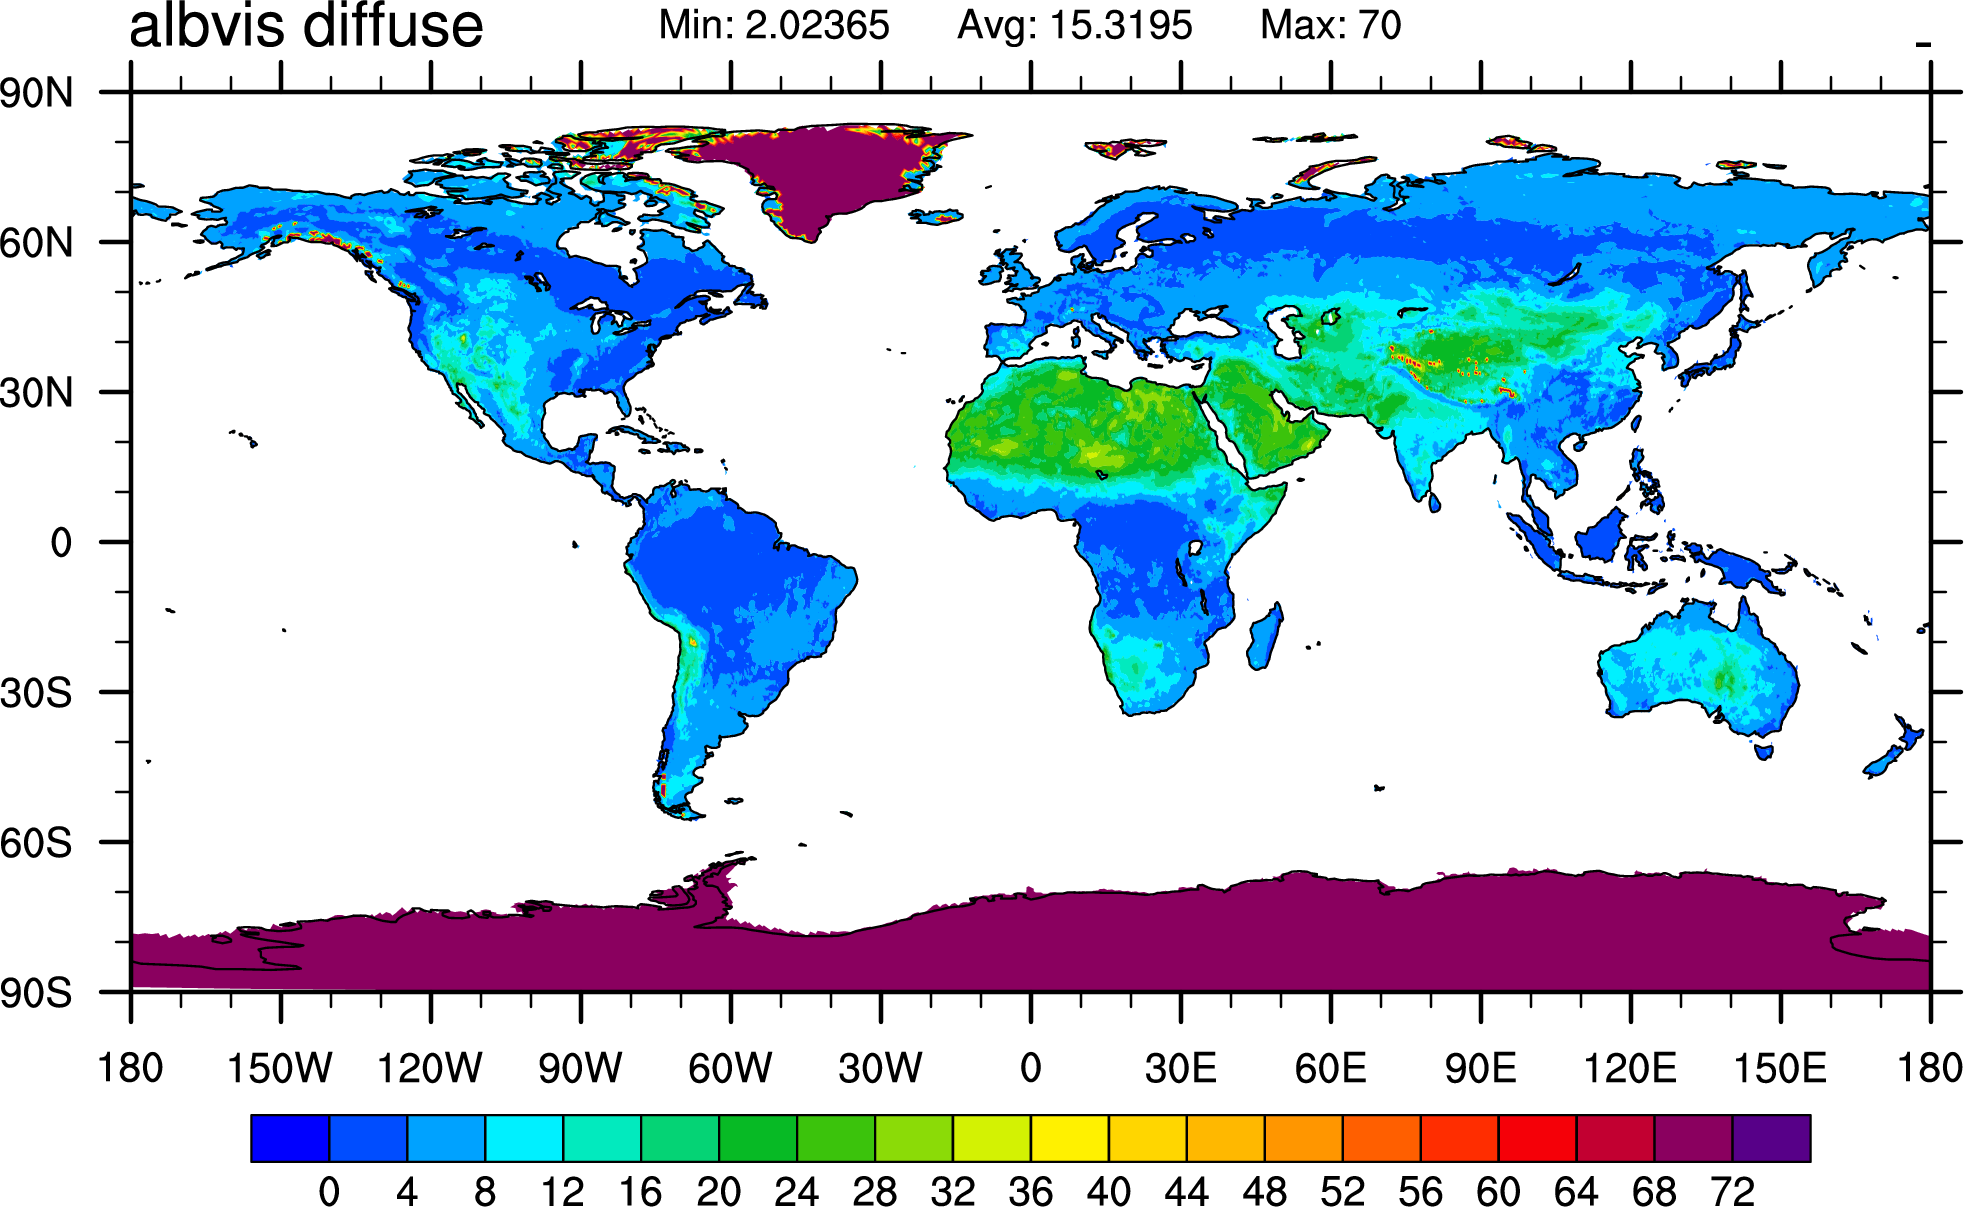
\includegraphics[width=8.1cm]{albvisdif_20120601_tuned.png}
  \end{minipage}
  \begin{minipage}[t]{0.498\textwidth}
    \center
    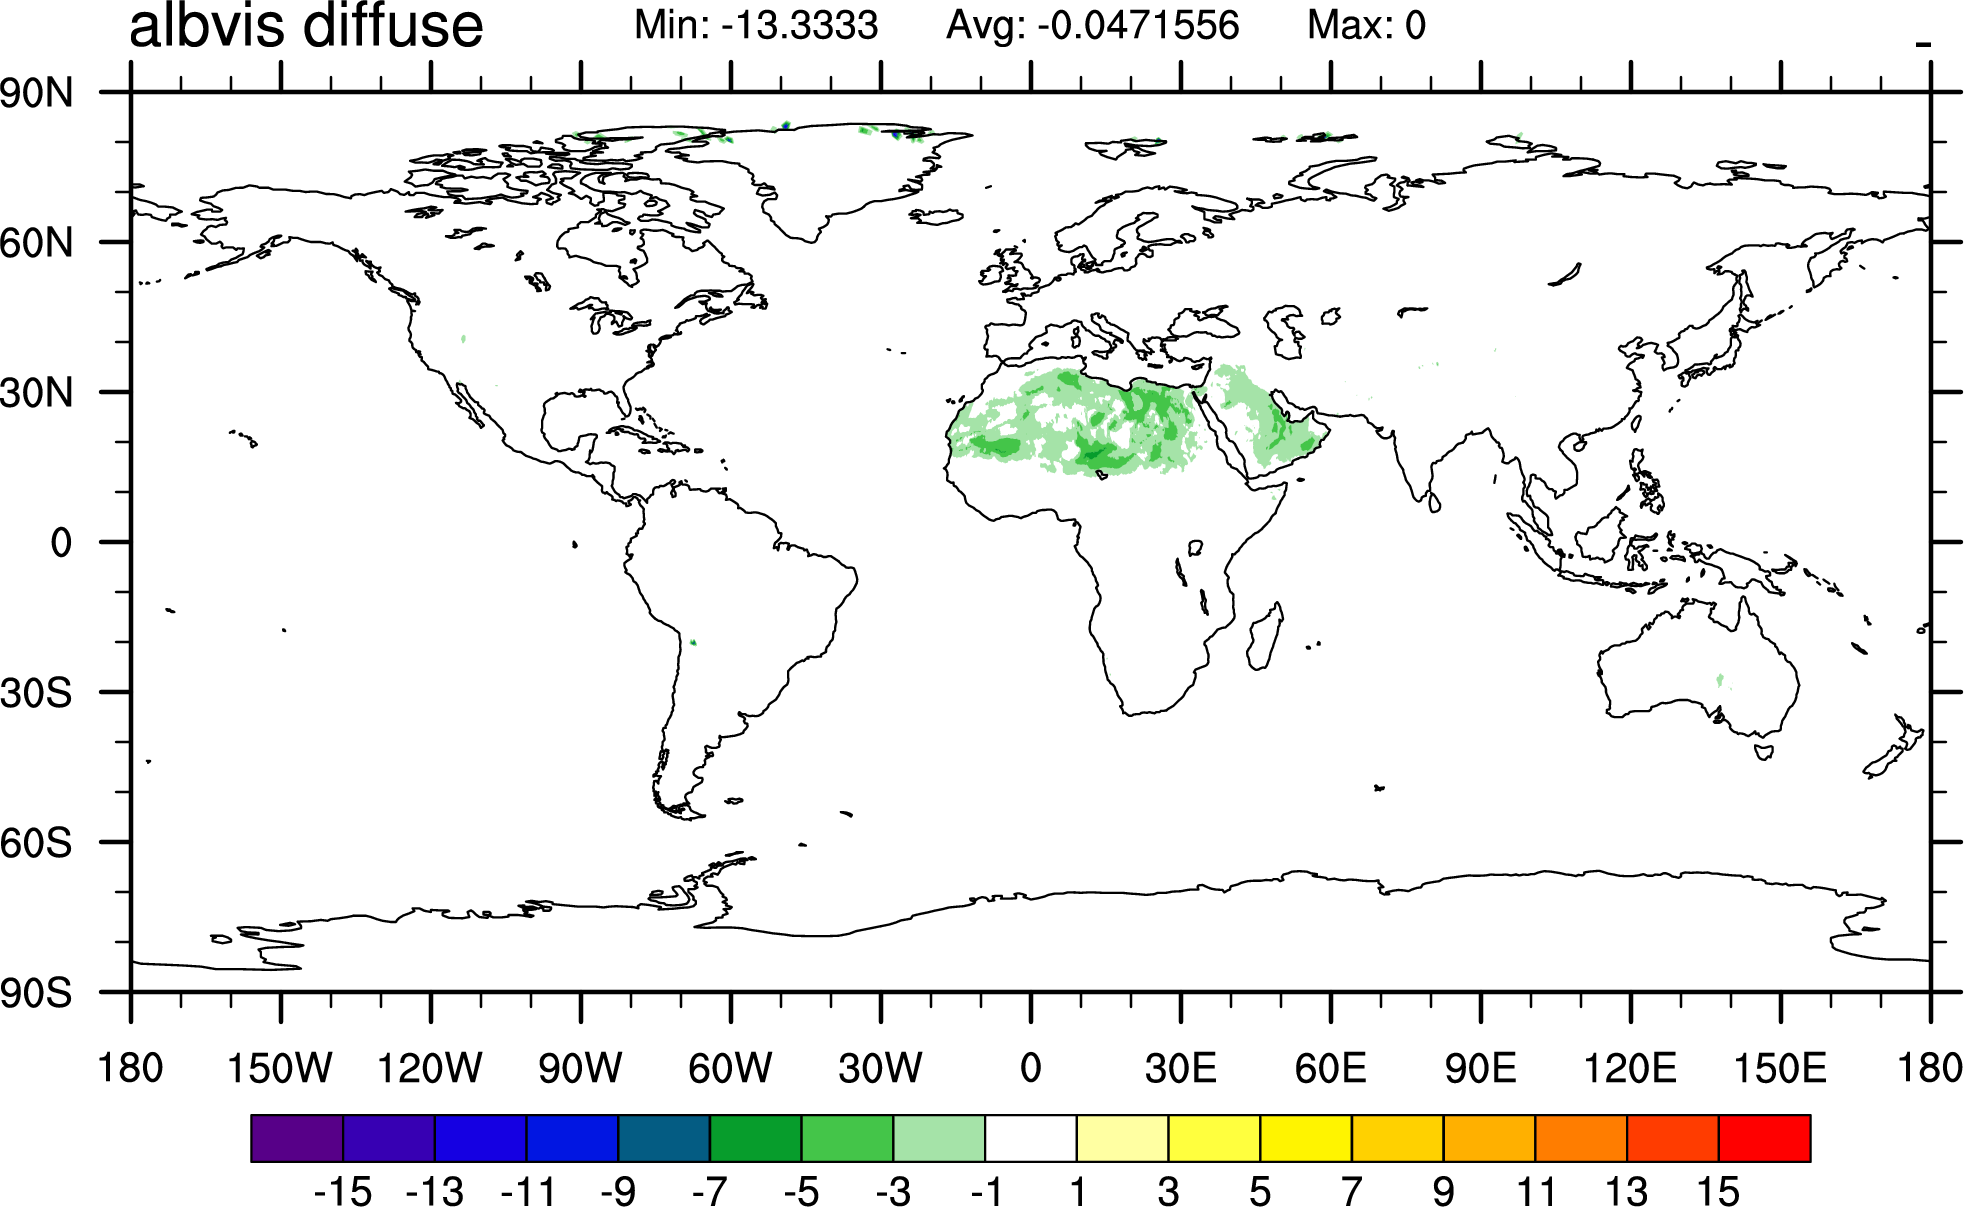
\includegraphics[width=8.1cm]{albvisdif_20120601_tuned-untuned.png}
  \end{minipage}
\end{minipage}
\caption{White sky (diffuse) albedo for UV-visible (left) spectral bands for the 1st June 2012 00UTC and its deviation from the original MODIS values (actual-original).}\label{fig_albvisdif}
\end{figure}

\begin{figure}[ht]
\begin{minipage}[t]{\textwidth}
  \begin{minipage}[t]{0.496\textwidth}
    \center
    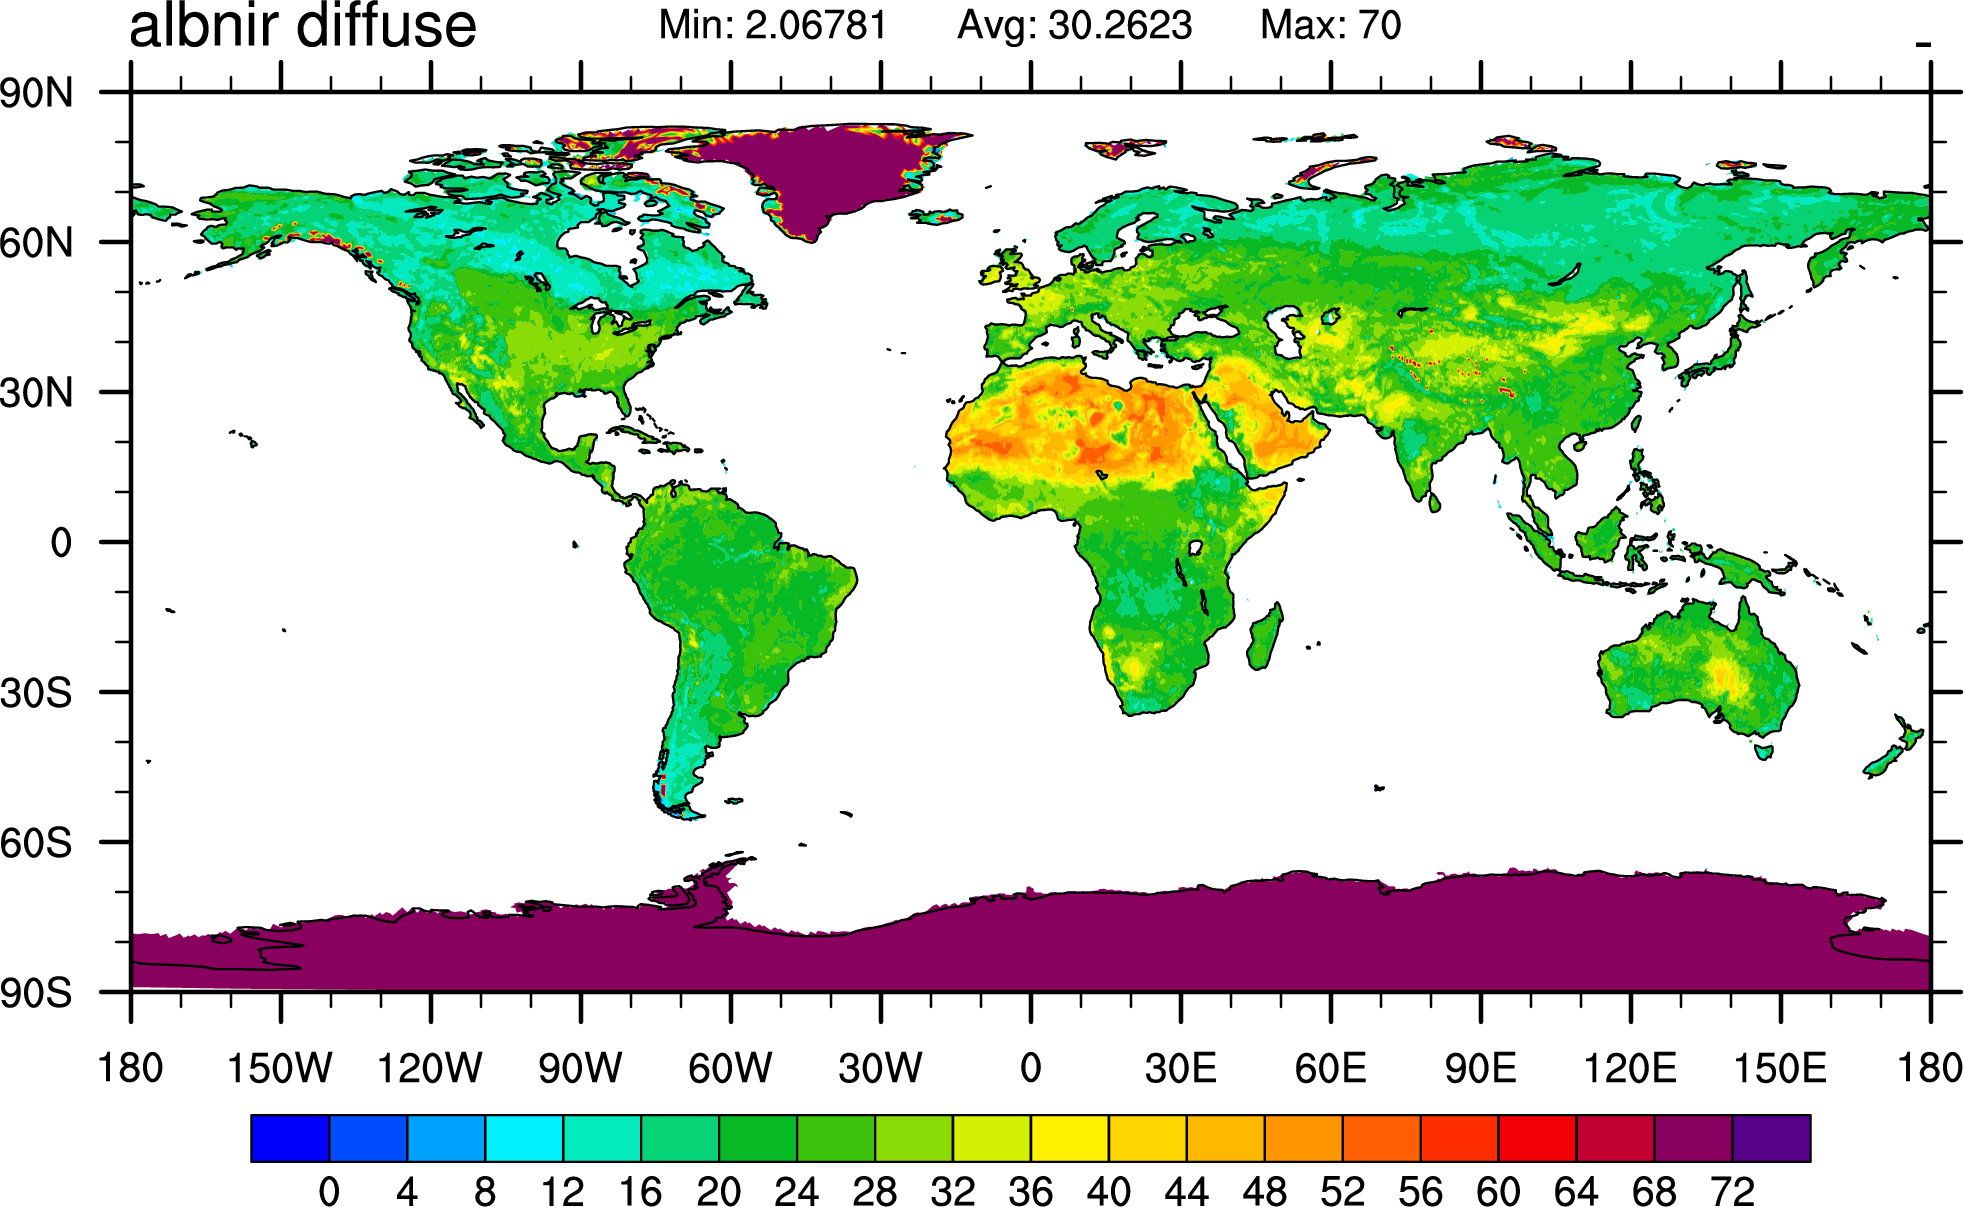
\includegraphics[width=7.7cm]{albnirdif_20120601_tuned.png}
  \end{minipage}
  \begin{minipage}[t]{0.496\textwidth}
    \center
    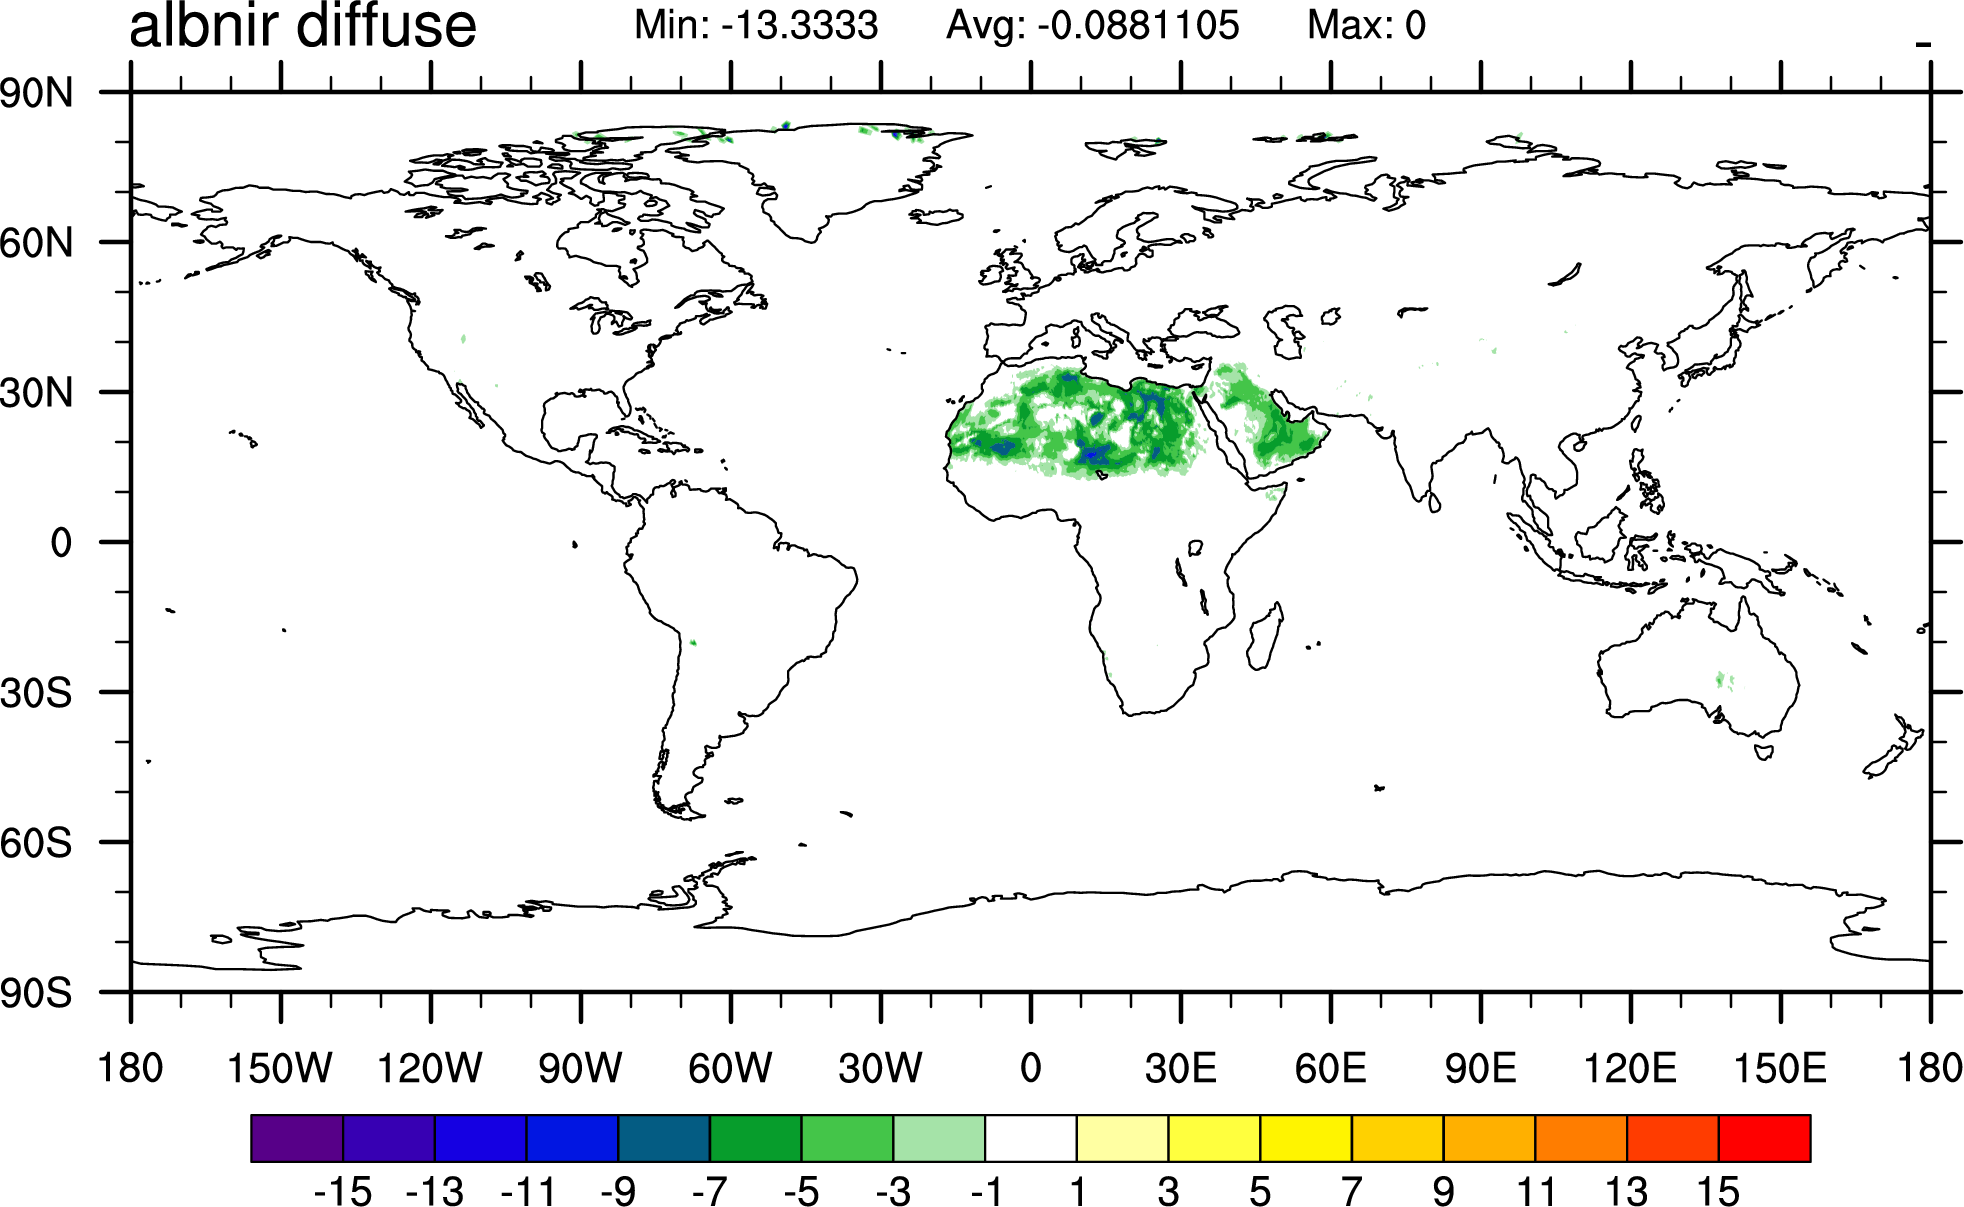
\includegraphics[width=7.7cm]{albnirdif_20120601_tuned-untuned.png}
  \end{minipage}
\end{minipage}
\caption{White sky (diffuse) albedo for near-infrared spectral bands (left) for the 1st June 2012 00UTC and its deviation from the original MODIS values (actual-original).}\label{fig_albnirdif}
\end{figure}



\subsection{Albedo for direct downward radiation (black sky)}
While the diffuse albedo does not depend on the solar zenith angle (SZA) $\theta_{0}$, direct albedo does \citep{Yang:2008}. 
Up to ICON-NWP version $2.0.05$ the formula for taking into account the zenith angle dependency was adapted from 
the Ritter-Geleyn radiation scheme. It was applied irrespective of the underlying surface type.
\begin{align}
  \alpha_{\mathrm{dir}}^{\lambda} = \frac{1.0 + 0.5\, \cos(\theta_{0})  \left(\frac{1}{\alpha_{\mathrm{diff}}^{\lambda}}-1\right)}
                              {\left[1.0 + \cos(\theta_{0})  \left(\frac{1}{\alpha_{\mathrm{diff}}^{\lambda}}-1\right)\right]^{2}} \label{eq:albdir_rg}
\end{align}
This parameterization was applied for both the UV-visible and near-infrared spectral bands. The functional dependency 
is visualized in Figure \ref{fig:albdir_ritter} for three different values of the diffuse albedo. At large solar zenith angles the 
direct albedo approaches $100\,\%$ irrespective of the diffuse albedo - a feature which is not supported by measurements.
Further note that the solar zenith angle at which $\alpha_{\rm dir}^{\lambda}=\alpha_{\rm diff}^{\lambda}$ decreases with increasing 
$\alpha_{\rm diff}^{\lambda}$. As far as we know this is not supported by albedo measurements.
\begin{figure}[hbt]
  \centering
  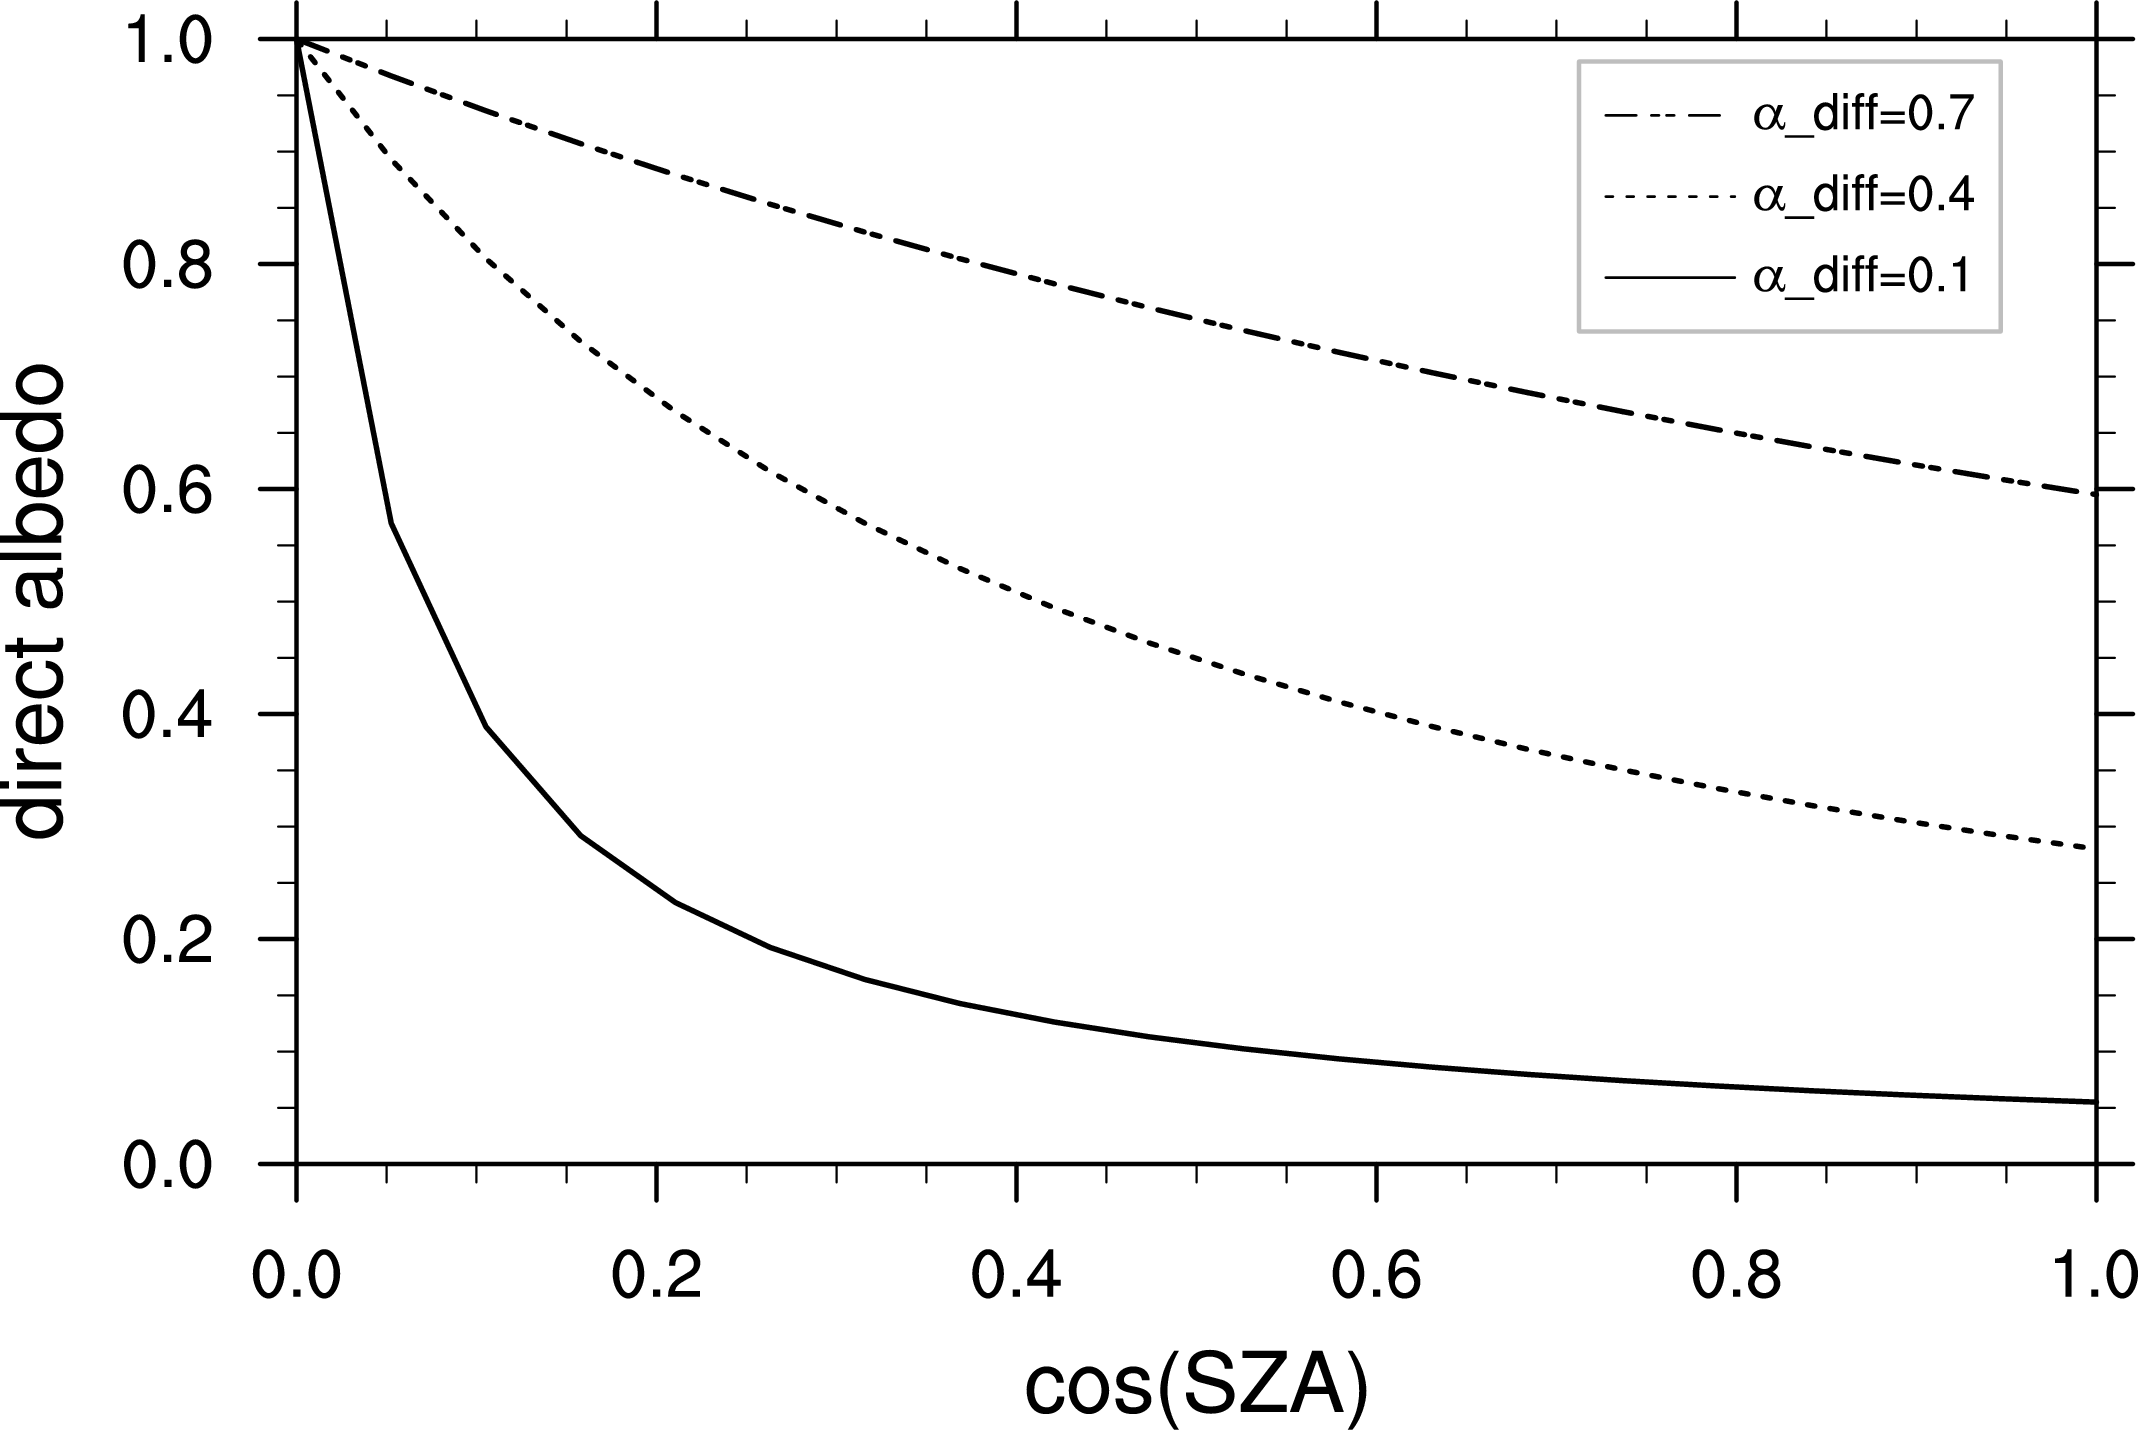
\includegraphics[width=12.0cm]{direct_albedo_Ritter.png}
  \caption{Solar zenith angle (SZA) dependence of the Black-sky (direct) albedo following Ritter (pers.\ comm.). Different lines 
  show functional the dependency for $3$ different values of the diffuse albedo. Note that the direct 
  albedo always reaches $1$ at $\theta_{0}=90^{\circ}$ zenith angle irrespective of the diffuse albedo.}\label{fig:albdir_ritter}
\end{figure}

From ICON-NWP version $2.0.06$ on, the parameterization \ref{eq:albdir_rg} is retained for water and ice points 
only. For snow-free land points a formulation following \cite{Briegleb82} is used.
\begin{align}
 \alpha_{\rm dir}^{\lambda} = \alpha_{\rm diff}^{\lambda}\, \frac{1.0 + d}{1.0 + 2.0 d \cos(\theta_{0})}\label{eq:albdir_Briegleb}
\end{align}
$d$ is a tuning constant taking into account that albedo can have a stronger or weaker dependence on SZA, depending on the surface 
type. In ICON we set
\begin{align}
 d= \begin{cases}
     0.4   &  \text{if $z_{0}\leq 0.15\,\mathrm{m}$}\\
     0.1   &  \text{if $z_{0} >  0.15\,\mathrm{m}$}\,,
    \end{cases}
\end{align}
meaning that a strong dependence on SZA is assumed for bare soil and low vegetation, while a weaker dependence is 
assumed for high vegetation (e.g.\ forests). The functional dependency is depicted in Figure \ref{fig:albdir_Briegleb}. 
Unlike the Ritter-Paratemerization, \cite{Briegleb82} assume 
$\alpha_{\rm dir}^{\lambda}(60^{\circ})= \alpha_{\rm diff}^{\lambda}$, which can easily be seen by inserting 
$\theta_{0}=60^{\circ}$ into equation \ref{eq:albdir_Briegleb}. This assumption is not too bad, but still only approximately true.
\begin{figure}[hbt]
  \centering
  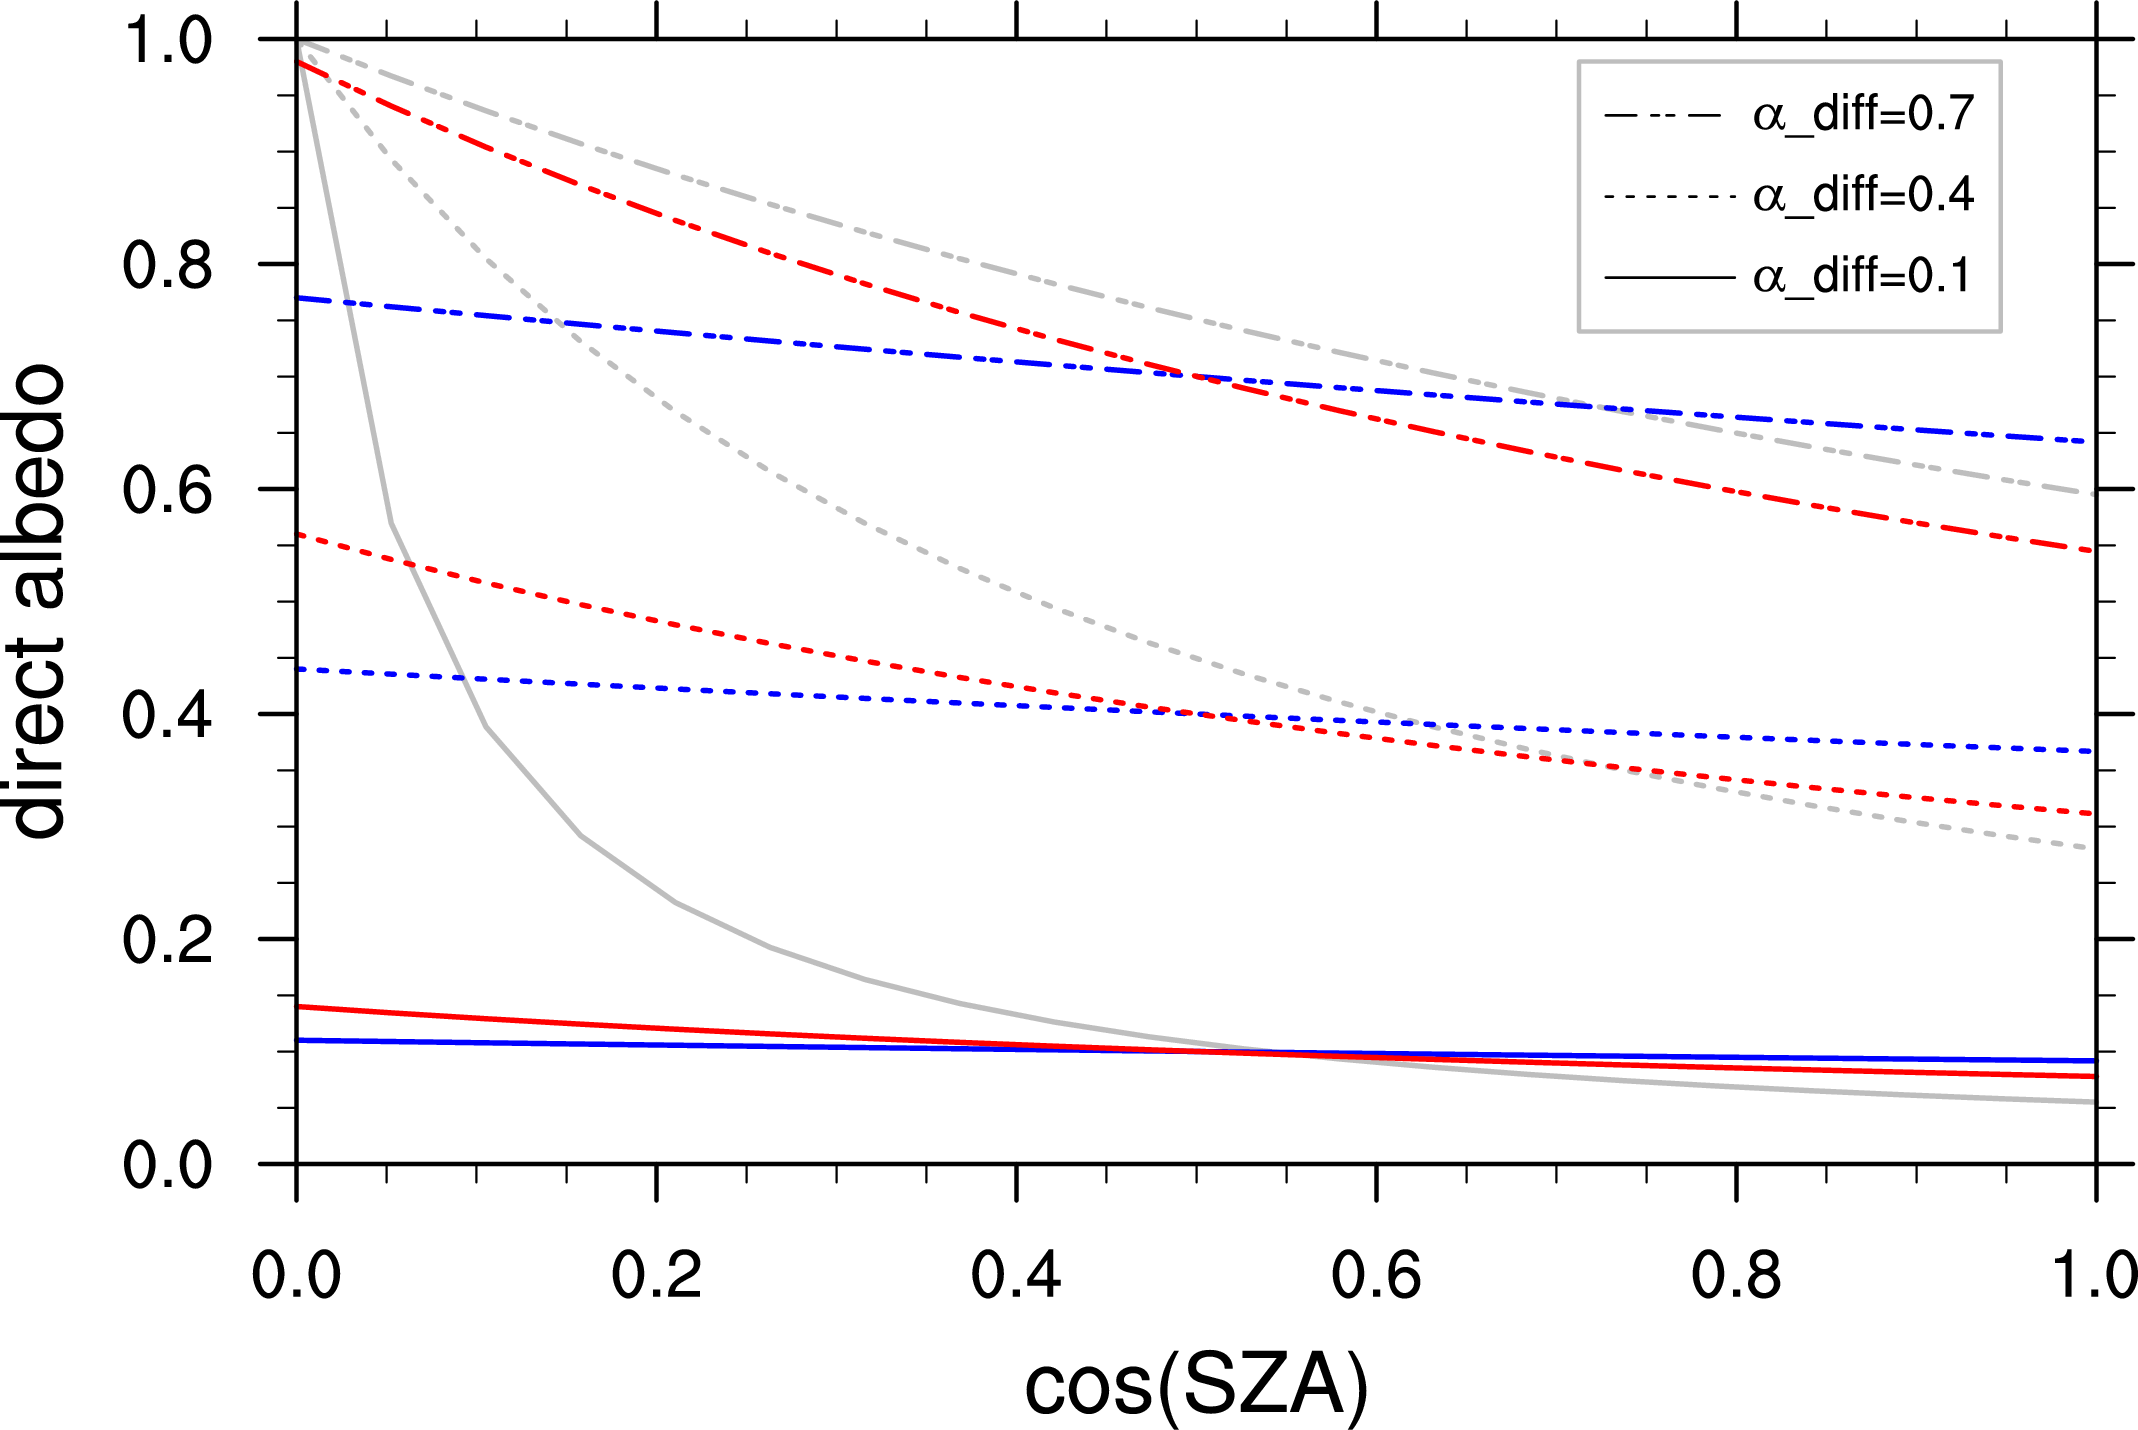
\includegraphics[width=12.0cm]{direct_albedo_Briegleb.png}
  \caption{Solar zenith angle (SZA) dependence of the Black-sky (direct) albedo following \cite{Briegleb82} 
  (equation \ref{eq:albdir_Briegleb}). Solid, dashed and long-dashed lines show the functional dependency for $3$ 
  different values of the diffuse albedo. Red lines show results assuming a strong ($d=0.4$) functional dependency, 
  while blue lines show results assuming a weak ($d=0.1$) functional dependency. Grey lines show the Ritter-parameterization 
  for comparison.}\label{fig:albdir_Briegleb}
\end{figure}

For snow-covered land points, we make use of modified Ritter-parameterization as proposed by Z\"angl 
(pers.\ comm.). Basically, the direct albedo is not allowed to exceed the diffuse albedo in cases with rough vegetation 
and/or mountainous regions. The direct albedo is estimated as follows:
\begin{align}
 \alpha_{\mathrm{dir}}^{\lambda} = \min\left[\alpha_{\mathrm{dir}^{\lambda}},\alpha_{\mathrm{dir}}^{\rm LIM}\right]
\end{align}
I.e.\ the direct albedo computed according to equation \eqref{eq:albdir_rg} is not allowed to exceed the 
limit $\alpha_{\mathrm{dir}}^{\rm LIM}$. The latter is defined as a weighted average of the unlimited direct  
albedo $\alpha_{\mathrm{dir}}^{\lambda}$ and the diffuse albedo $\alpha_{\mathrm{diff}}^{\lambda}$.
\begin{align}
 \alpha_{\mathrm{dir}}^{\rm LIM} = \gamma \cdot \alpha_{\mathrm{diff}}^{\lambda} + (1-\gamma)\cdot \alpha_{\mathrm{dir}}^{\lambda}
\end{align}
The limit tends towards $\alpha_{\mathrm{diff}}^{\lambda}$ the more rough the surface or orography at the given grid point is. 
The weighting factor $\gamma$ is parameterized as a function of the SSO standard deviation $\sigma_{SSO}$ and 
the landuse class specific roughness length $z_{0}$. $\gamma$ is close to $0$ for landuse classes with 'smooth' vegetation/ orography 
and becomes $1$ for $z_{0}>0.15\,\mathrm{m}$ or $\sigma_{SSO}>150\,\mathrm{m}$.
\begin{align}
 \gamma &= \max\left[0.01\cdot (\sigma_{SSO}-50),10\cdot(z_{0}-0.05)\right]\\
 \gamma &= \min(1,\max(0,\gamma))
\end{align}
The functional dependency is depicted in Figure \ref{fig:albdir_Zaengl}.
\begin{figure}[hbt]
  \centering
  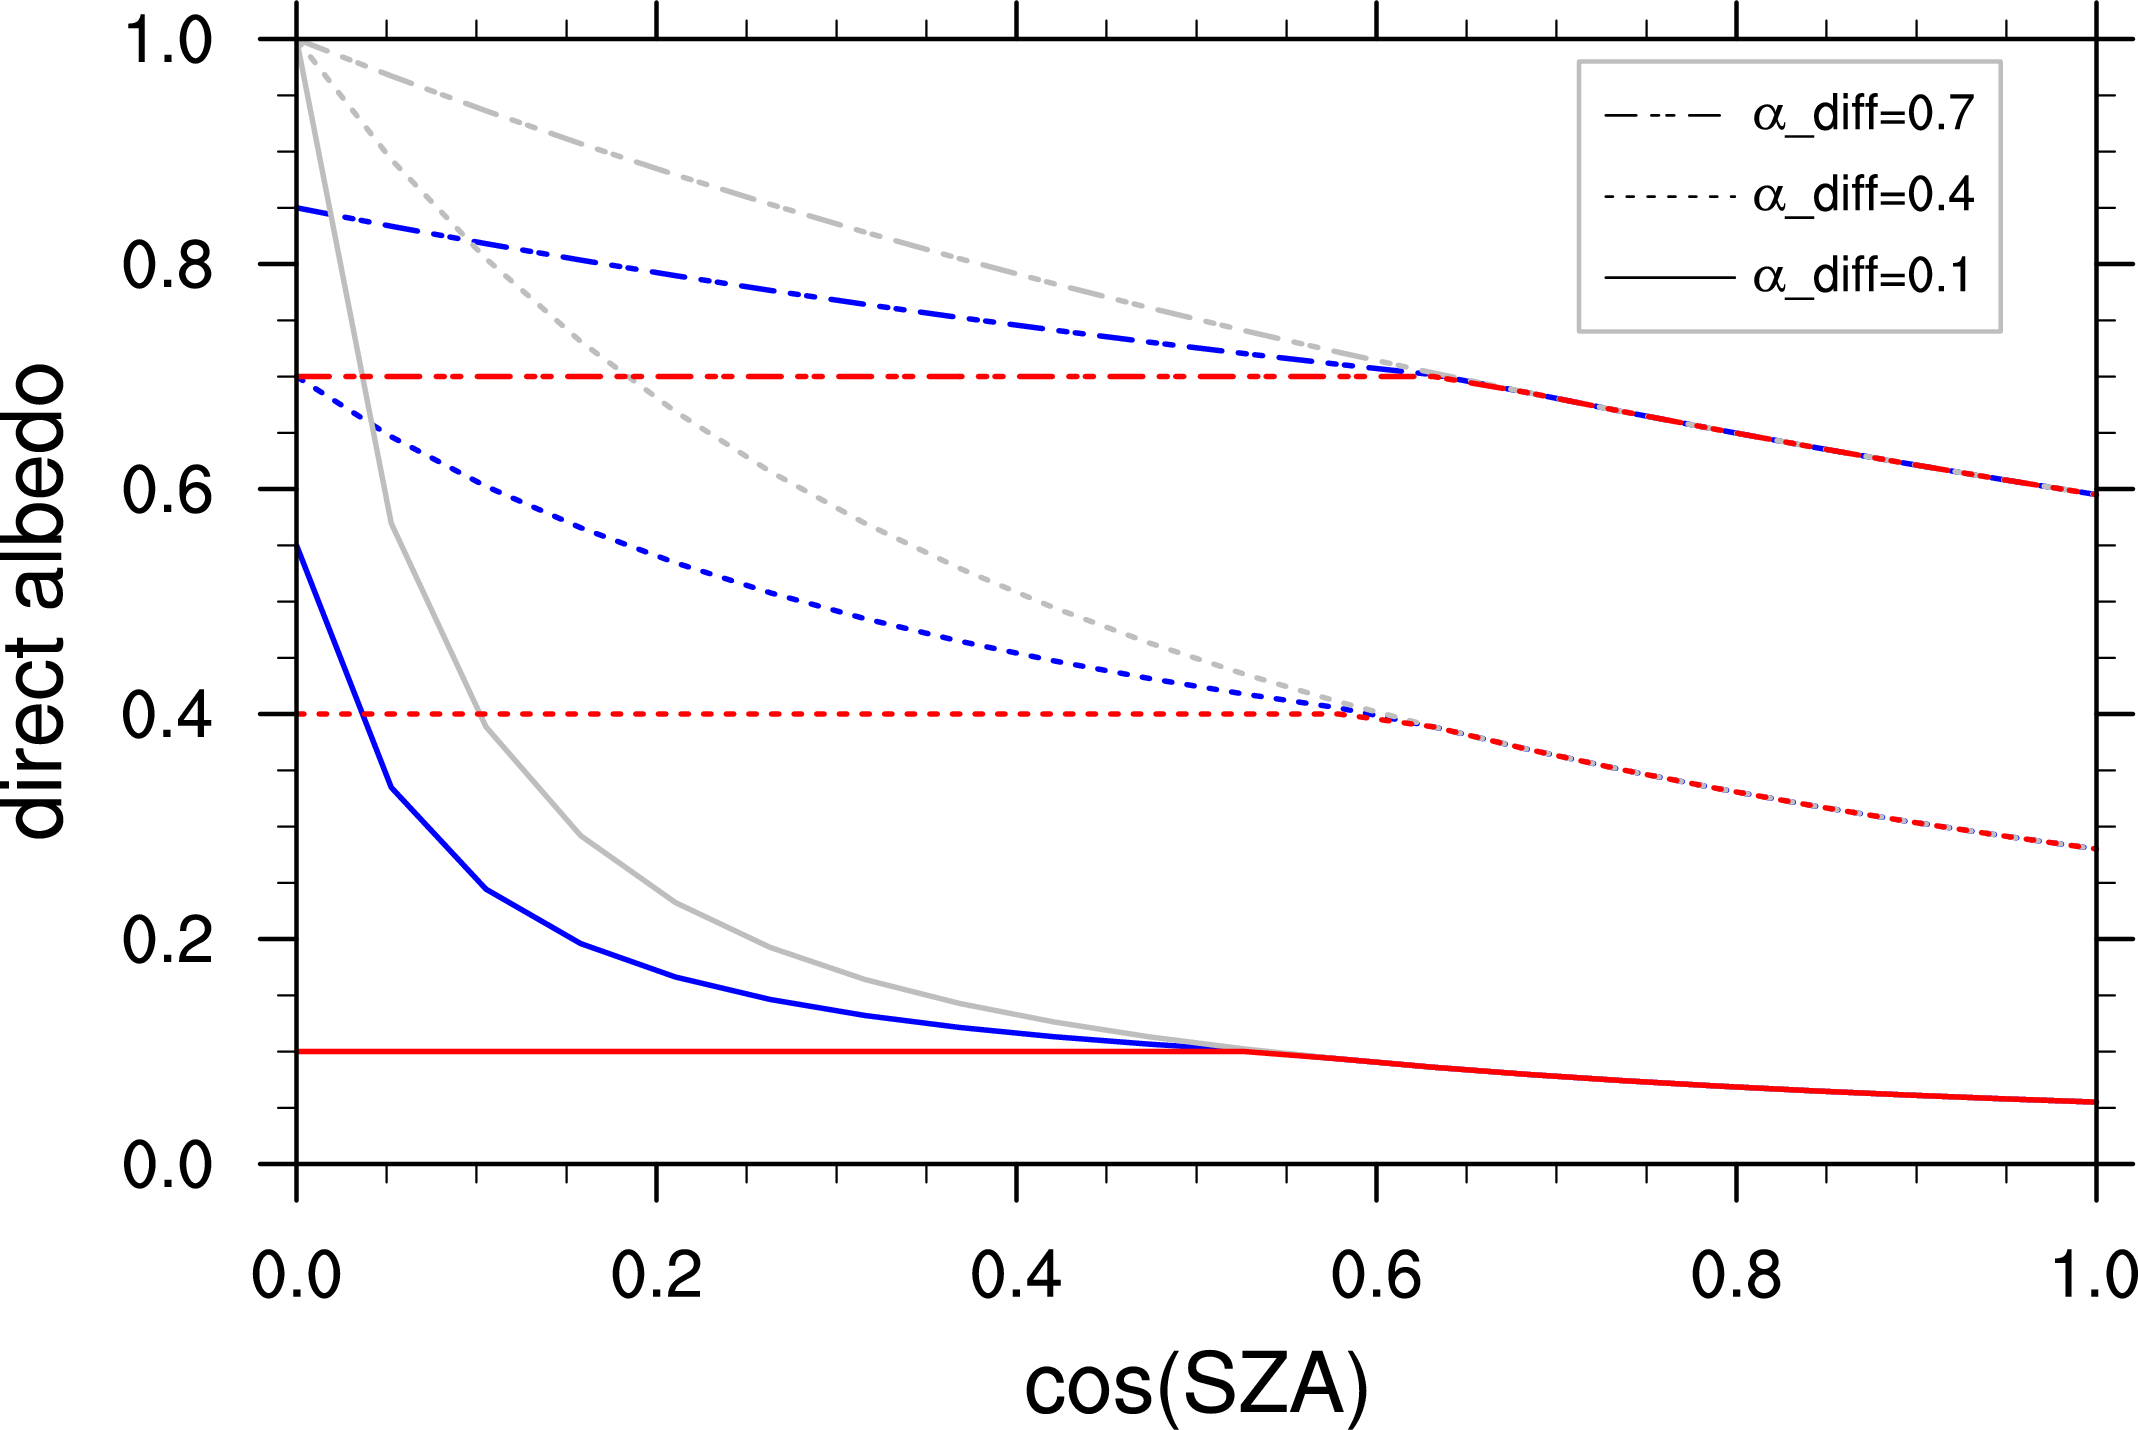
\includegraphics[width=12.0cm]{direct_albedo_Zaengl.png}
  \caption{Solar zenith angle (SZA) dependence of the Black-sky (direct) albedo following Z\"angl, as it is currently 
  used for snow-covered points. Solid, dashed and long-dashed lines show functional dependency for $3$ different 
  values of the  diffuse albedo. Blue lines show results assuming a roughness length of $z_{0}=0.1$. Red lines are 
  valid for $z_{0}=1.0$. For comparison the Ritter-Parameterization is shown in grey.}\label{fig:albdir_Zaengl}
\end{figure}


An example for 1st June 2012 04UTC, based on the diffuse albedos shown in Figure \ref{fig_albvisdif} and \ref{fig_albnirdif} is given in Figure \ref{fig_albdir}. 
\begin{figure}[hbt]
\begin{minipage}[t]{\textwidth}
  \begin{minipage}[t]{0.498\textwidth}
    \center
    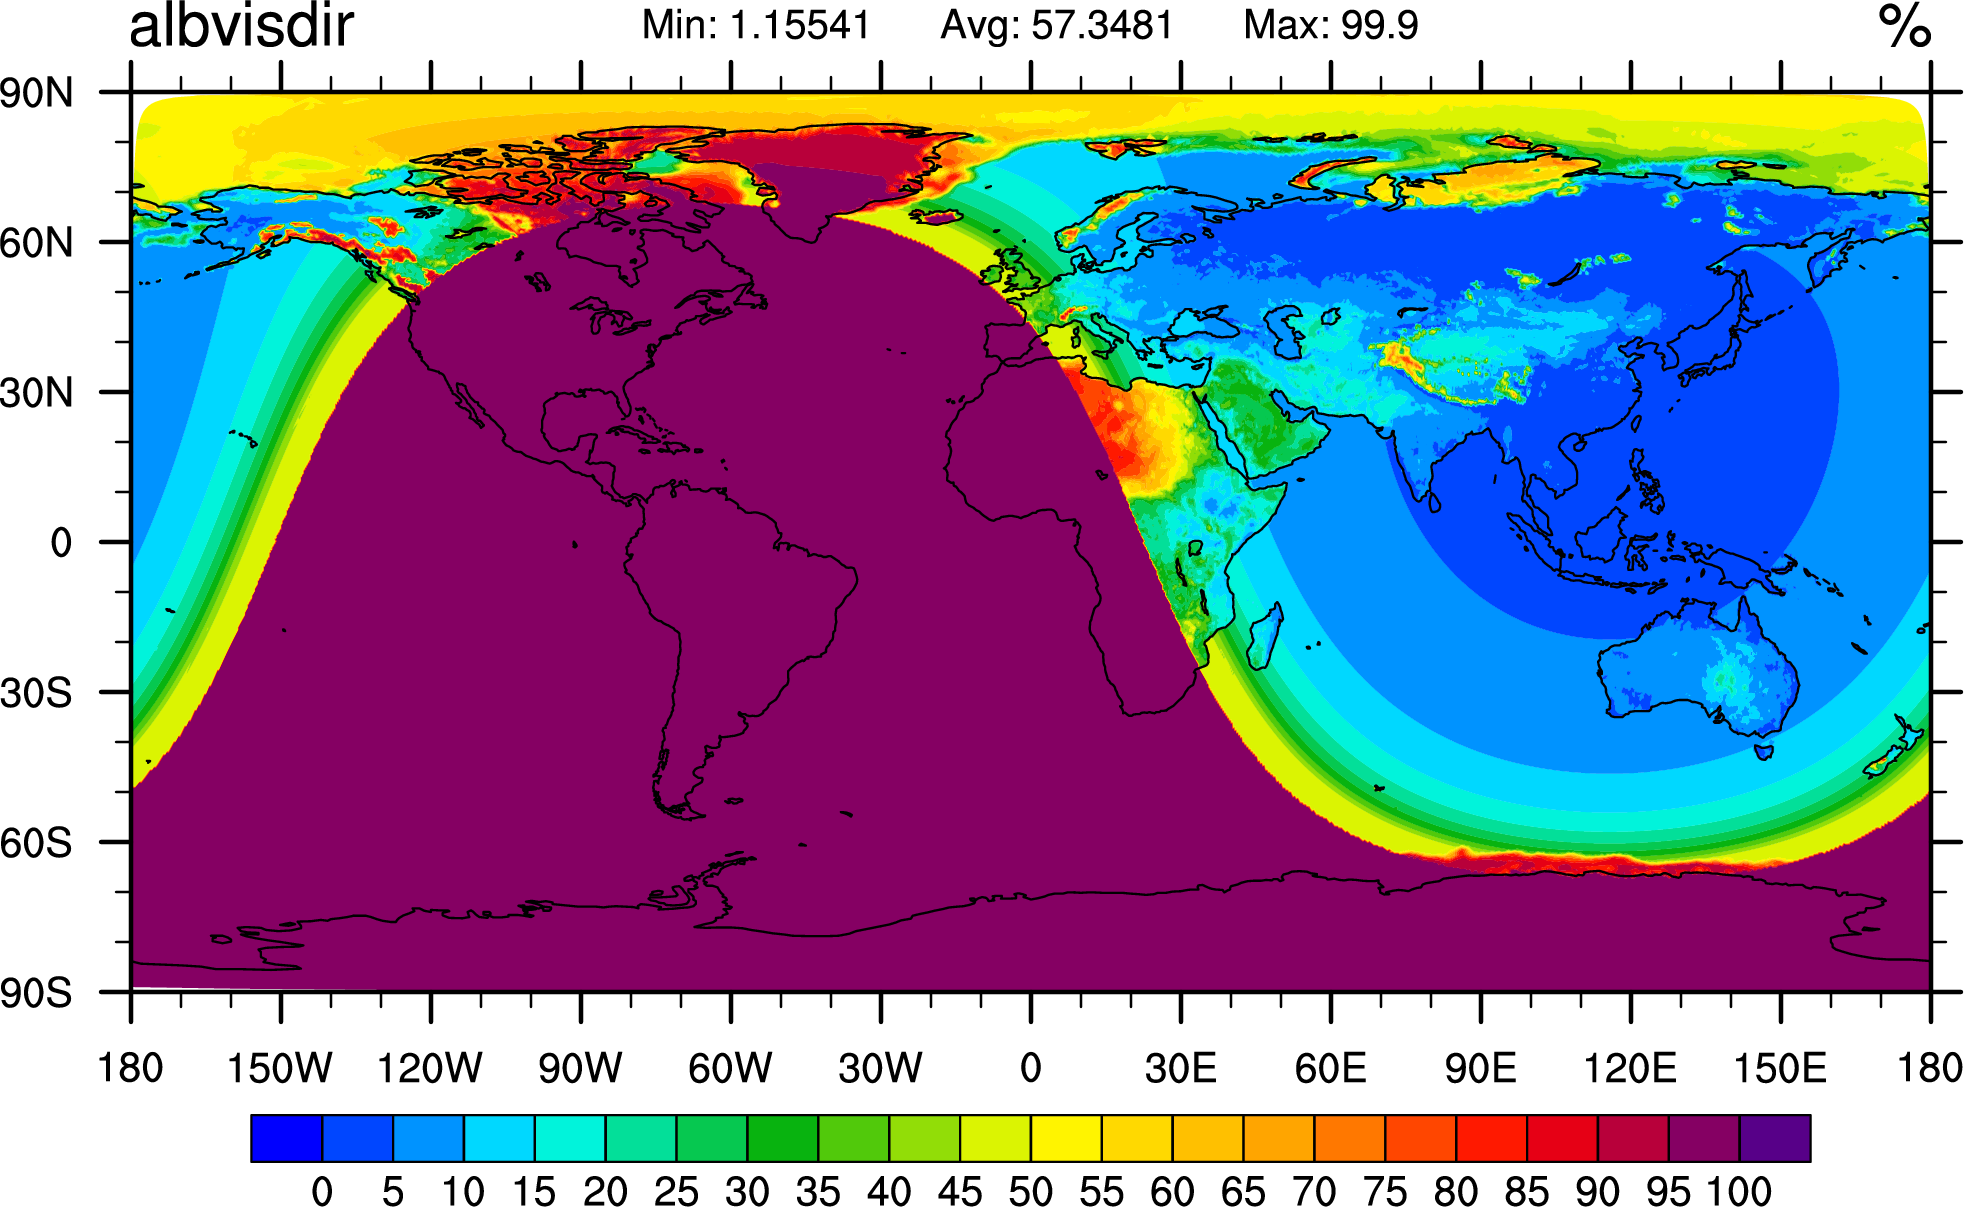
\includegraphics[width=8.1cm]{albvisdir_20120601_blacksky_ritter.png}
  \end{minipage}
  \begin{minipage}[t]{0.498\textwidth}
    \center
    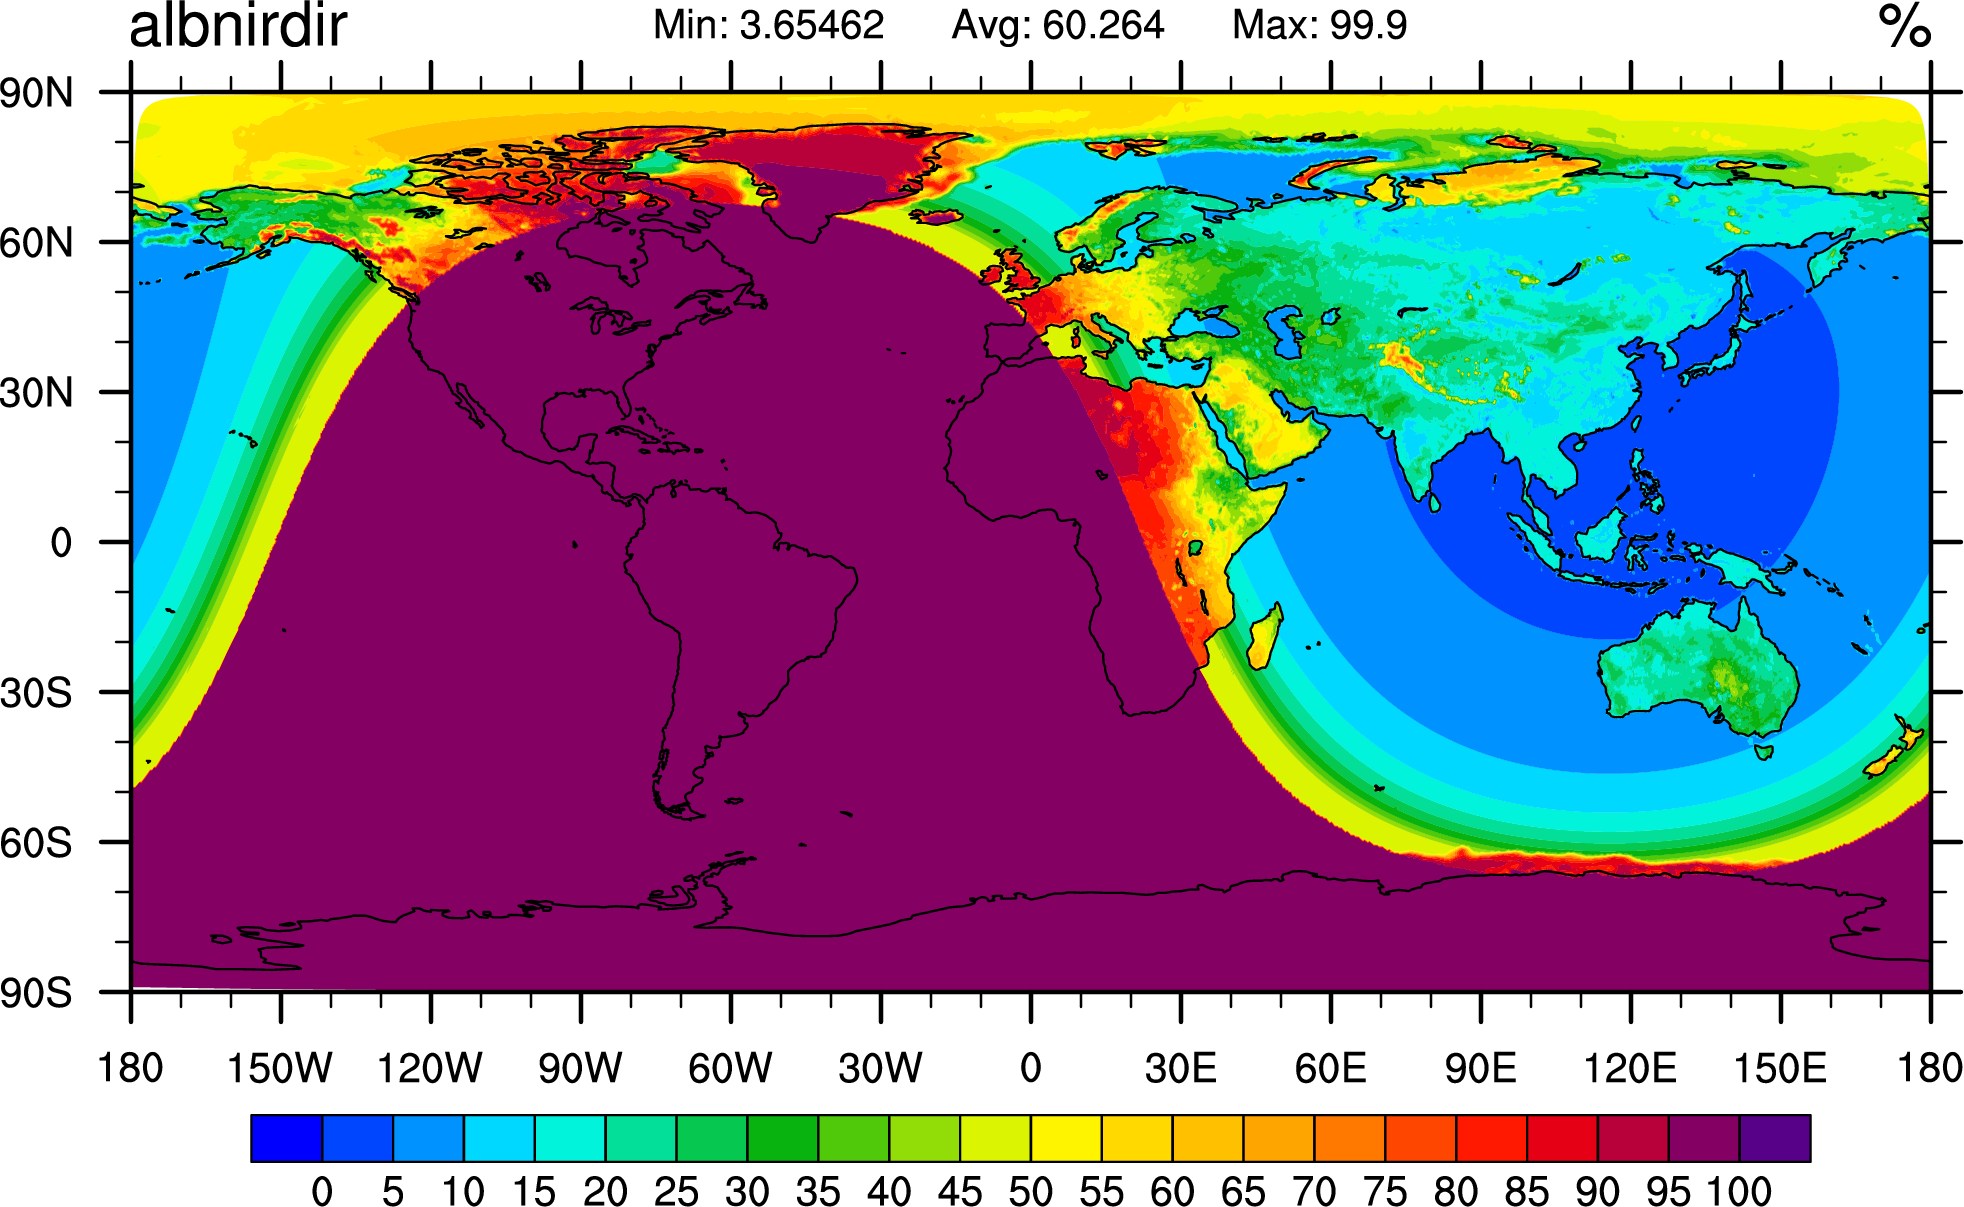
\includegraphics[width=8.2cm]{albnirdir_20120601_blacksky_ritter.png}
  \end{minipage}
\end{minipage}
\caption{Black sky (direct) albedo for UV-visible (left) and near-infrared (right) spectral bands for the 4th Jan 2012 04UTC.}\label{fig_albdir}
\end{figure}

% \subsubsection{Sample plots}
% Figure \ref{fig_albvisdif} and \ref{fig_albnirdif} show the white sky surface albedo (UV-visible and near-infrared) for the 1st June 2012 00UTC as it is 
% operationally used by ICON for snow-free land points. Note that compared to the original MODIS data, the Saharan albedo has been slightly reduced in order 
% to compensate for a model cold bias in that region.
% 
% \begin{figure}[ht]
% \begin{minipage}[t]{\textwidth}
%   \begin{minipage}[t]{0.498\textwidth}
%     \center
%     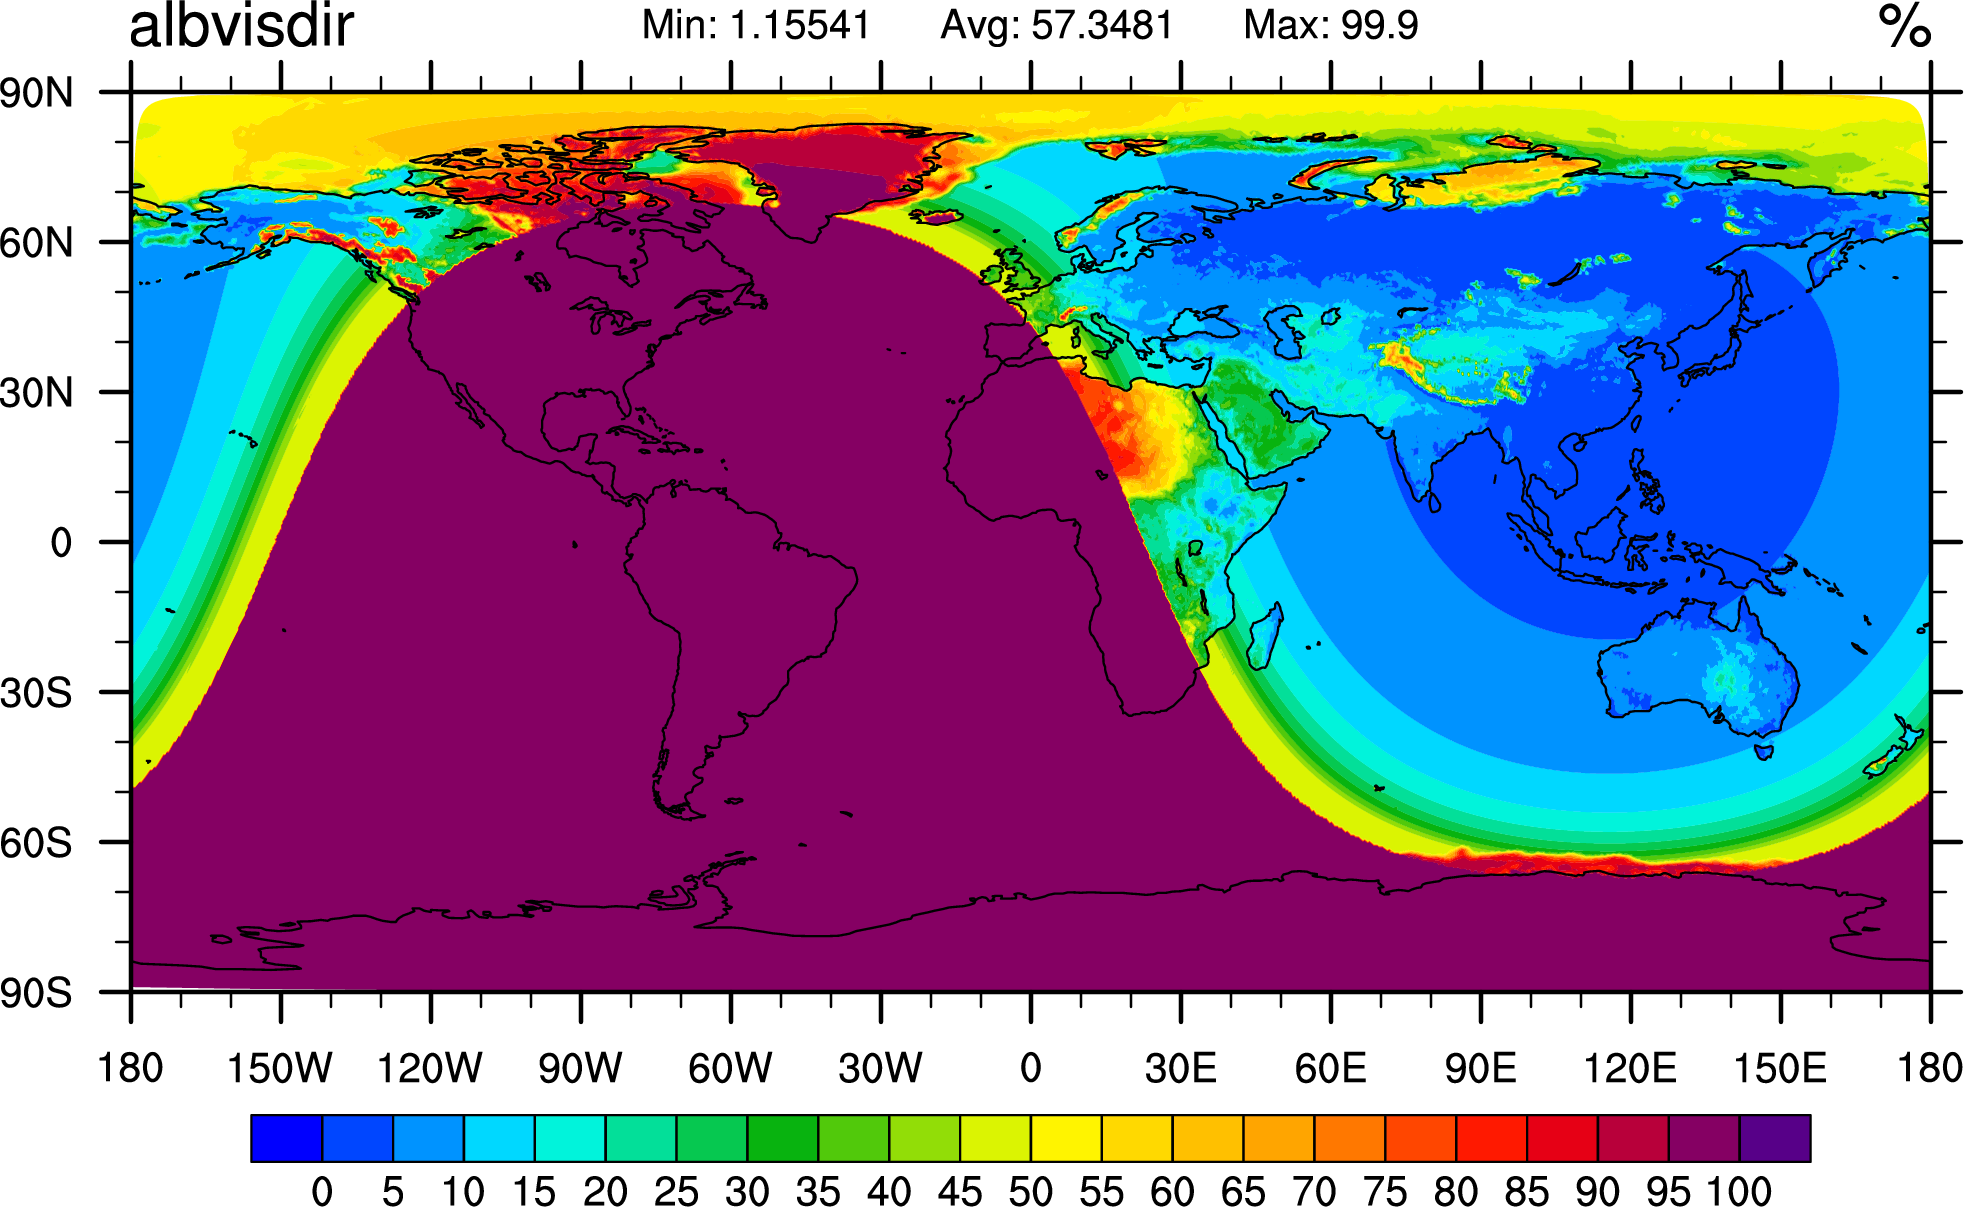
\includegraphics[width=8.1cm]{albvisdir_20120601_blacksky_ritter.png}
%   \end{minipage}
%   \begin{minipage}[t]{0.498\textwidth}
%     \center
%     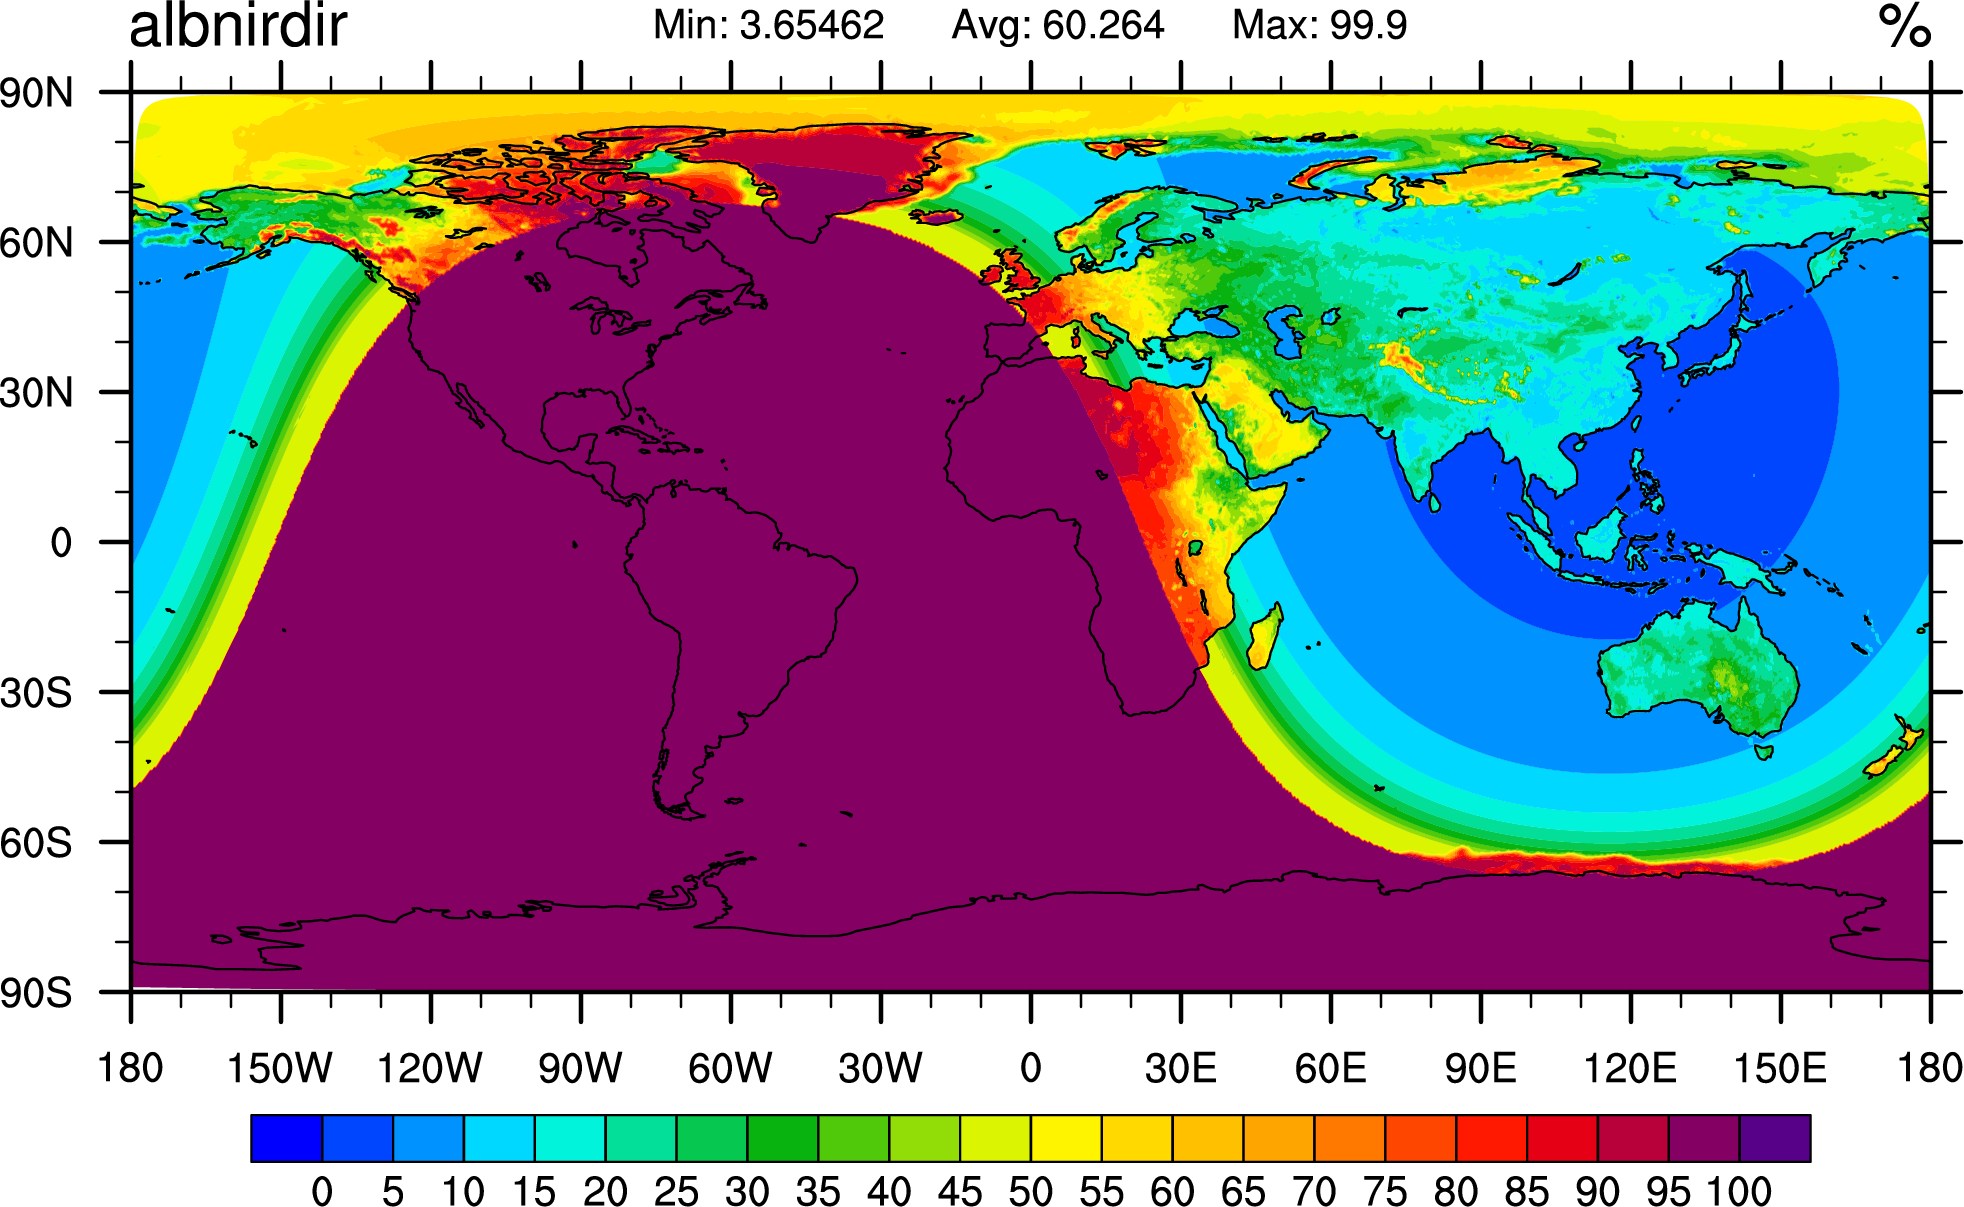
\includegraphics[width=8.2cm]{albnirdir_20120601_blacksky_ritter.png}
%   \end{minipage}
% \end{minipage}
% \caption{Black sky (direct) albedo for UV-visible (left) and near-infrared (right) spectral bands for the 4th Jan 2012 00UTC.}\label{fig_albdir}
% \end{figure}

%-------------------------------------------------------------------------

\bibliography {../references-icon-science}
\bibliographystyle {../wileyqj} %QJ


\end{document}
